%%%%%%%%%%%%%%%%%%%%%%%%%%%%%%%%%%%%%%%%%%%%%%%%%%%%%%%%%%%%%%
\fe{\section{Calcul thermique}}{\section{Thermal Calculation}}
\label{thermique}
%%%%%%%%%%%%%%%%%%%%%%%%%%%%%%%%%%%%%%%%%%%%%%%%%%%%%%%%%%%%%%

\begin{frame}{\fe{Thermique}{Thermal analysis}}{\fe{Rappels}{Reminders}}
  \begin{itemize}
    \item \fe{Équation de la chaleur}{Heat equation}
    \begin{block}{\fe{Forme locale}{Local form}}
      \begin{equation*}
        \rho c_p \frac{\partial T}{\partial t}+\tx{div}\underbrace{\left(-\lambda\ve{\tx{grad}}(T)\right)}_{\ve{\phi}}=q\quad\fe{\tx{sur }V}{\tx{on }V}
      \end{equation*}
    \end{block}
    \footnotesize
    \fe{avec :}{with:}
    \begin{itemize}
      \begin{columns}
        \begin{column}{.4\textwidth}
          \item[] $T$ \fe{température}{temperature}
          \item[] $\ve{\phi}$ \fe{densité de flux de chaleur}{heat flow density}
          \item[] $q$ \fe{source de chaleur volumique}{volumic heat source}
        \end{column}
        \begin{column}{.42\textwidth}
          \item[] $\lambda$ \fe{conductivité thermique}{thermal conductivity}
          \item[] $\rho$ \fe{masse volumique}{mass density}
          \item[] $c_p$ \fe{capacité thermique massique}{Massic heat capacity}
          \item[] $t$ \fe{temps}{time}
        \end{column}
      \end{columns}
    \end{itemize}
    \normalsize
    \item \fe{Conditions aux limites}{Boundary conditions}\\
    \footnotesize
    \fe{Températures imposées}{Imposed temperatures}
    $T=T_{\tx{imp}}$ \fe{sur $\partial V_T$}{on $\partial V_T$}\\
    \fe{Flux imposés}{Imposed heat flow}
    $\ve{\phi}.\ve{n}=\phi_{\tx{imp}}+\underbrace{h(T_f-T)}_{\tx{convection}}+\underbrace{\varepsilon \sigma(T_\infty^4-T^4)}_{\tx{\fe{rayonnement}{radiation}}}$
    \fe{sur $\partial V_{\phi}$}{on $\partial V_{\phi}$}
    \normalsize
  \end{itemize}
\end{frame}

\begin{frame}{\fe{Thermique}{Thermal analysis}}{\fe{Rappels}{Reminders}}
  \begin{itemize}
    \item \fe{Éléments finis :}{Finite elements:}
    \footnotesize
    \begin{center}
      $T(x)=[N(x)]\{T\}$ \qquad $\ve{\tx{grad}}(T)=[B(x)]\{T\}$
    \end{center}
    \normalsize
    \begin{block}{\fe{Formulation faible et discrétisée :}
                     {Weak and discrete formulation:}}
      \begin{equation*}
        [C]\{\dot{T}\}+[K]\{T\}=\{P\}
      \end{equation*}
    \end{block}~\\
    \footnotesize
    \fe{avec les matrices :}{with the matrices:}
    \begin{tabular}{ll}~\\
      $[C]=\int_V\rho c_p [N]^T[N]dV$ & \fe{matrice de capacité}{capacity matrix}\\
      $[K]=\int_V[B]^T[\lambda][B]dV+\int_{\partial V_{\phi}}h[N]^T[N]dS$ & \fe{matrice de conductivité}{conductivity matrix}
     \end{tabular}~\\~\\
    \fe{et le vecteur chargement nodal équivalent :}{and the equivalent nodal load vector:}
    \begin{itemize}
      \item[] $\{P\}=\int_V[N]^TqdV+\int_{\partial V_{\phi}}[N]^T(\phi_{\tx{imp}}+hT_f+\varepsilon\sigma(T_\infty^4-T^4))dS$
    \end{itemize}
    \normalsize
  \end{itemize}
\end{frame}

\begin{frame}{\fe{2.1 Problème étudié}{2.1 Problem description}}
  \begin{itemize}
    \item \fe{Conduction, régime stationaire}{Conduction, steady state}
    \begin{center}
    \footnotesize
    \begin{tikzpicture}
      \node[anchor=south west,inner sep=0] (image) at (0,0)
      {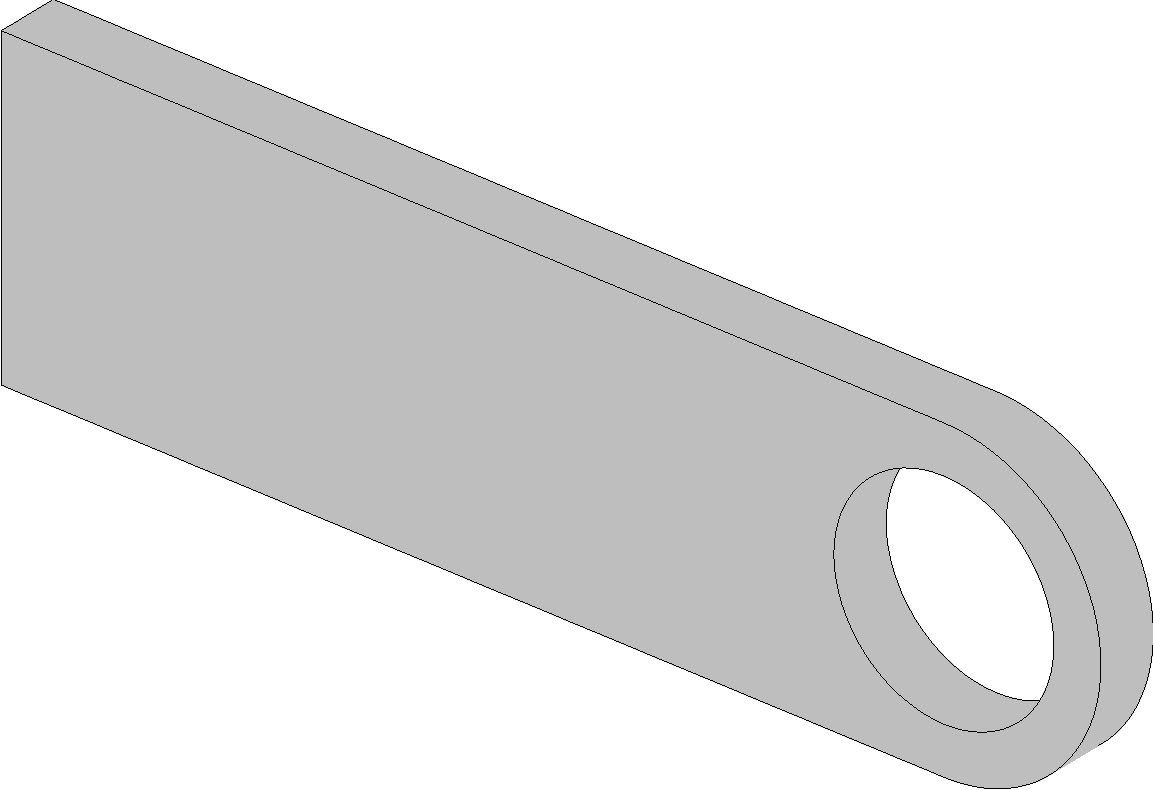
\includegraphics[width=4cm]{images/exo/1.2_geometrie}};
      \begin{scope}[x={(image.south east)},y={(image.north west)}]
        \draw (1,0.9) node[anchor=west] {$\lambda$~=~50~W.m$^{-1}$.K$^{-1}$};
        \draw (1,0.7) node[anchor=west] {$c_p$~=~420~J.K$^{-1}$.kg$^{-1}$};
        \draw (1,0.5) node[anchor=west] {$\rho$~=~7800~kg.m$^{-3}$};
        \draw (1,0.2) node[anchor=west] {$T_{t=0}$~=~0~°C};
      \end{scope}
    \end{tikzpicture}
    \normalsize
    \end{center}
    \begin{columns}
      \begin{column}{.4\textwidth}
        \item \fe{Température imposée}{Imposed temperature}
        \footnotesize
        \begin{tikzpicture}
          \node[anchor=south west,inner sep=0] (image) at (0,0)
          {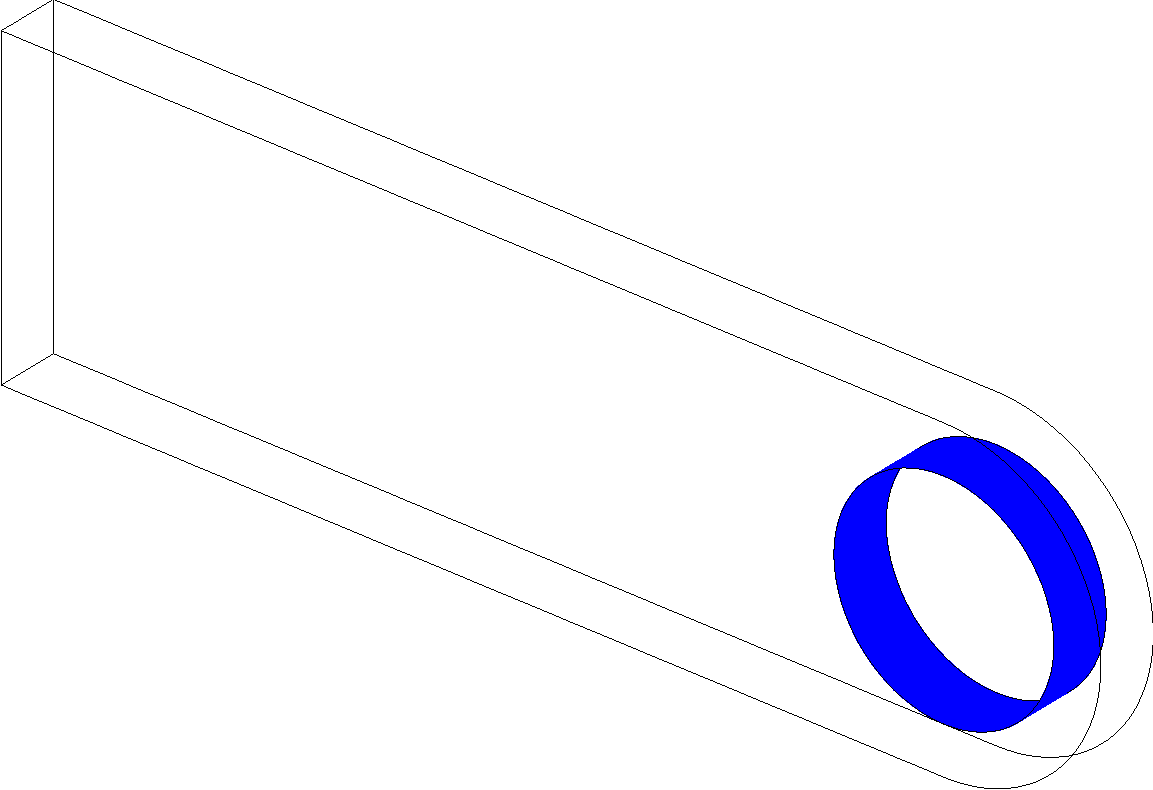
\includegraphics[width=3.5cm]{images/exo/2.1_cl_temperature}};
          \begin{scope}[x={(image.south east)},y={(image.north west)},color=blue]
            \draw (0.8,0.66) node[anchor=north west] {$T$~=~250~°C};
          \end{scope}
        \end{tikzpicture}
        \normalsize
      \end{column}
      \begin{column}{.4\textwidth}
        \item \fe{Flux de chaleur imposé}{Imposed heat flow}
        \footnotesize
        \begin{tikzpicture}
          \node[anchor=south west,inner sep=0] (image) at (0,0)
          {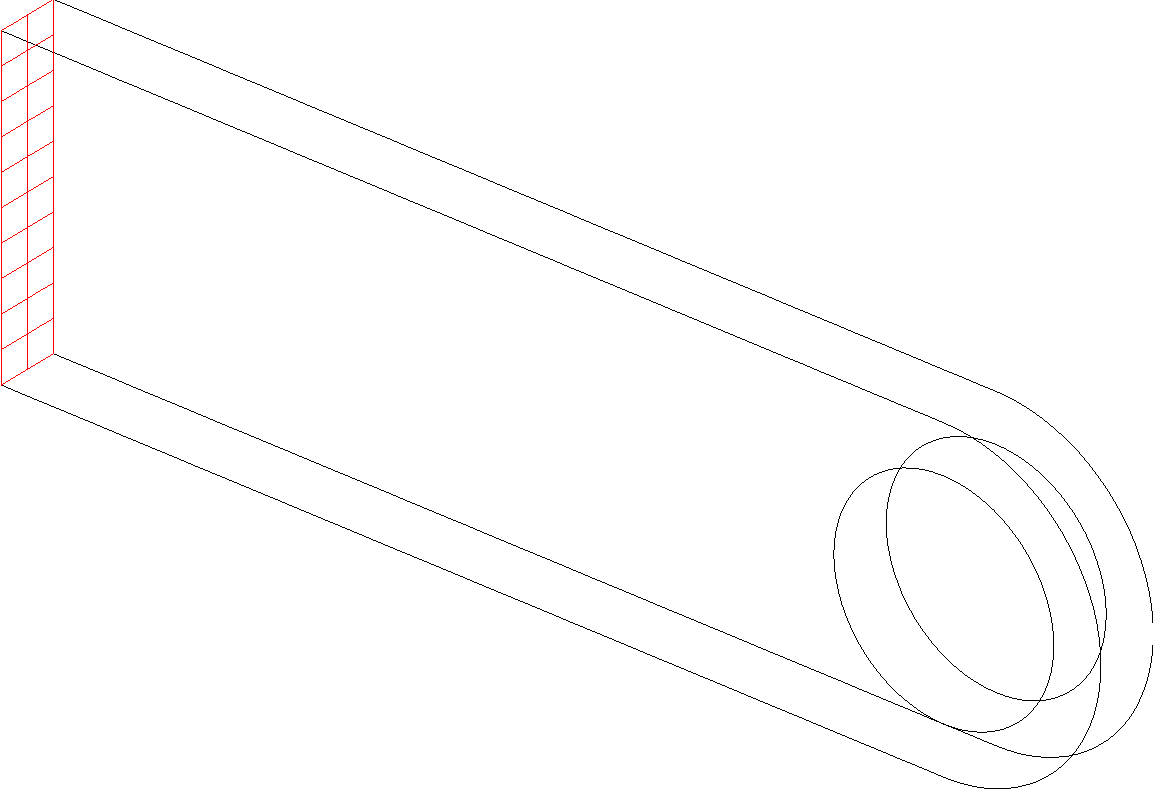
\includegraphics[width=3.5cm]{images/exo/2.1_cl_flux}};
          \begin{scope}[x={(image.south east)},y={(image.north west)},color=red]
            \draw (-0.25,0.5) node[anchor=north west,fill=white] {$\phi$~=~-40~kW.m$^{-2}$};
          \end{scope}
        \end{tikzpicture}
        \normalsize
      \end{column}
    \end{columns}
  \end{itemize}
\end{frame}

\begin{frame}{\fe{2.1 Thermique linéaire}{2.1 Linear thermal analysis}}
             {\fe{Stationnaire, conduction}{Steady state, conduction}}
  \begin{itemize}
    \item \fe{Objectif : calcul thermique stationnaire\\
              en températures et flux imposés}
            {Objective: steady state thermal calculation\\
             with fixed temperatures and heat flow}
    \begin{center}
      $\gray{[C]\{\dot{T}\}}+[K]\{T\}=\{P\}$ \qquad $\Rightarrow$ \fe{Système linéaire}{Linear system}
    \end{center}
    \item \fe{Méthode :}{Method:}\\
    \begin{tabular}{ll}
      \fe{calcul de la matrice de conductivité}{conductivity matrix calculation} & $[K]$\\
      \fe{calcul des chargement nodaux équivalents}{fixed nodal heat loads calculation} & $\{P\}$\\
      \fe{résolution avec \kwr{RESO}}{sovling with \kwr{RESO}} & $\{T\}$
    \end{tabular}
  \end{itemize}
\end{frame}

\begin{frame}{\fe{2.1 Thermique linéaire}{2.1 Linear thermal analysis}}
             {\fe{Stationnaire, conduction}{Steady state, conduction}}
  \begin{itemize}
    \item \fe{Restitution des objets (maillage, paramètres, …)}
             {Input data from previous computation (mesh, parameters, …)}
    \lstinputlisting[language=gibiane, firstline=30, lastline=31]{dgibi/formation_debutant_2_thermique.dgibi}
    \avous{\fe{Tous les objets sauvegardés sont chargés en mémoire\\
               \quad~Ils sont alors accessibles de suite}
              {All of the objects are loaded into memory\\
               \quad~~~They can be called now}}
    \item \fe{Noveaux paramètres}{New parameters}
    \lstinputlisting[language=gibiane, firstline=44, lastline=47]{dgibi/formation_debutant_2_thermique.dgibi}
    \lstinputlisting[language=gibiane, firstline=49, lastline=53]{dgibi/formation_debutant_2_thermique.dgibi}
  \end{itemize}
\end{frame}

\begin{frame}{\fe{2.1 Thermique linéaire}{2.1 Linear thermal analysis}}
             {\fe{Stationnaire, conduction}{Steady state, conduction}}
  \begin{itemize}
    \item \fe{Formulation mathématique (conduction)}{Mathematical formulation (conduction)}
    \lstinputlisting[language=gibiane, firstline=79, lastline=81]{dgibi/formation_debutant_2_thermique.dgibi}
    \item<2->\fe{Matrice de conductivité}{Conductivity matrix}
    \onslide<2->{
      \lstinputlisting[language=gibiane, firstline=83, lastline=84]{dgibi/formation_debutant_2_thermique.dgibi}
      \begin{flushright}
        \footnotesize
        $[K]=\int_V[B]^T[\lambda][B]dV+\gray{\int_{\partial V_{\phi}}h[N]^T[N]dS}$
        \normalsize
      \end{flushright}
      \vspace{2cm}}
    \item[]<2->\violet{\emph{\fe{Nouveaux objets :}{New objects:} MMODEL, MCHAML, RIGIDITE}}
  \end{itemize}
\end{frame}

\begin{frame}{\fe{2.1 Thermique linéaire}{2.1 Linear thermal analysis}}
             {\fe{Stationnaire, conduction}{Steady state, conduction}}
  \begin{itemize}
    \item \fe{Conditions aux limites}{Boundary conditions}
    \lstinputlisting[language=gibiane, firstline=86, lastline=91]{dgibi/formation_debutant_2_thermique.dgibi}
    \lstinputlisting[language=gibiane, firstline=96, lastline=96]{dgibi/formation_debutant_2_thermique.dgibi}
    \begin{textblock*}{5cm}(8.6cm,-2.6cm)
      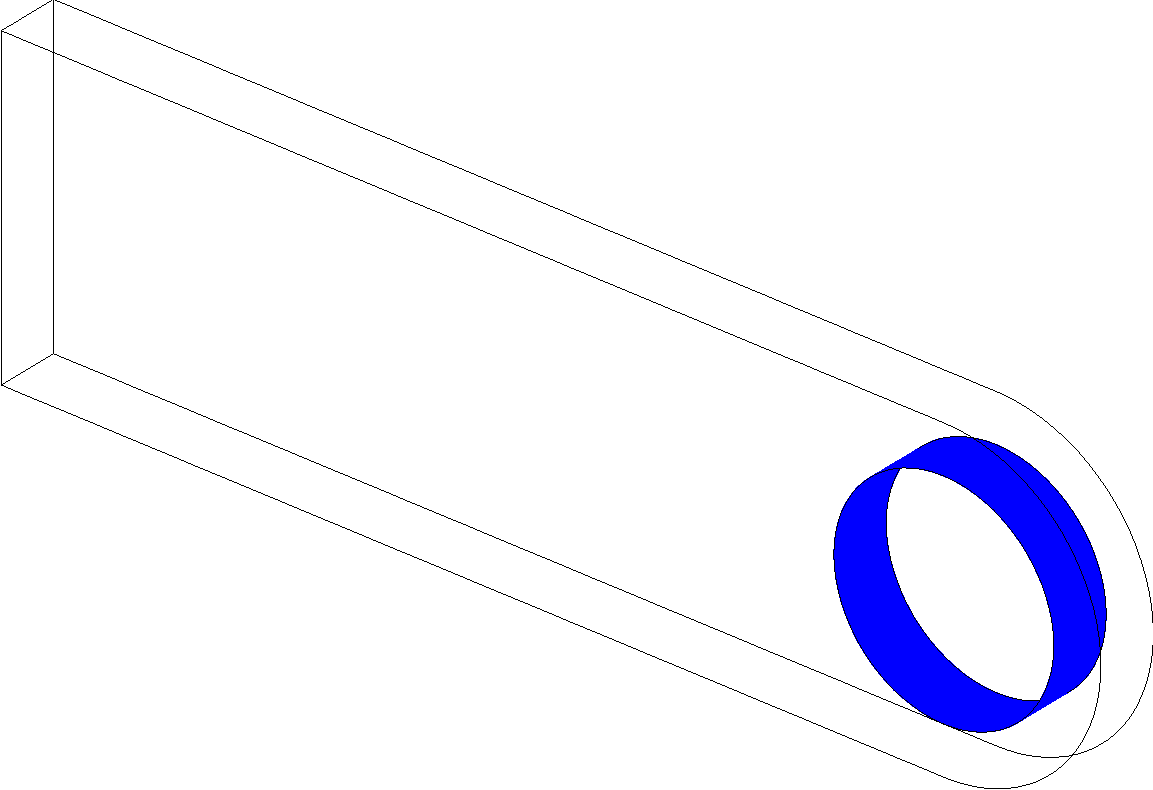
\includegraphics[width=3.5cm]{images/exo/2.1_cl_temperature}
    \end{textblock*}
    \onslide<2->{
      \lstinputlisting[language=gibiane, firstline=103, lastline=108]{dgibi/formation_debutant_2_thermique.dgibi}}
    \onslide<3->{
      \lstinputlisting[language=gibiane, firstline=110, lastline=112]{dgibi/formation_debutant_2_thermique.dgibi}
      \begin{flushright}
        \footnotesize
        $\{P\}=\gray{\int_V[N]^TqdV}+\int_{\partial V_{\phi}}[N]^T(\phi_{\tx{imp}}\gray{+hT_f+\varepsilon\sigma(T_\infty^4-T^4)})dS$
        \normalsize
      \end{flushright}}
  \end{itemize}
\end{frame}

\begin{frame}{\fe{2.1 Thermique linéaire}{2.1 Linear thermal analysis}}
             {\fe{Stationnaire, conduction}{Steady state, conduction}}
  \begin{itemize}
    \item \fe{Résolution et affichage des résultats}{Solving and plotting results}
    \lstinputlisting[language=gibiane, firstline=114, lastline=115]{dgibi/formation_debutant_2_thermique.dgibi}
    \onslide<2->{\lstinputlisting[language=gibiane, firstline=122, lastline=122]{dgibi/formation_debutant_2_thermique.dgibi}}
    \onslide<3->{\lstinputlisting[language=gibiane, firstline=123, lastline=123]{dgibi/formation_debutant_2_thermique.dgibi}}
    \onslide<4->{\lstinputlisting[language=gibiane, firstline=125, lastline=125]{dgibi/formation_debutant_2_thermique.dgibi}}
    \onslide<4->{\lstinputlisting[language=gibiane, firstline=127, lastline=127]{dgibi/formation_debutant_2_thermique.dgibi}}
    \vspace{3cm}
    \onslide<2>{
      \begin{textblock*}{6cm}(6cm,-4cm)
        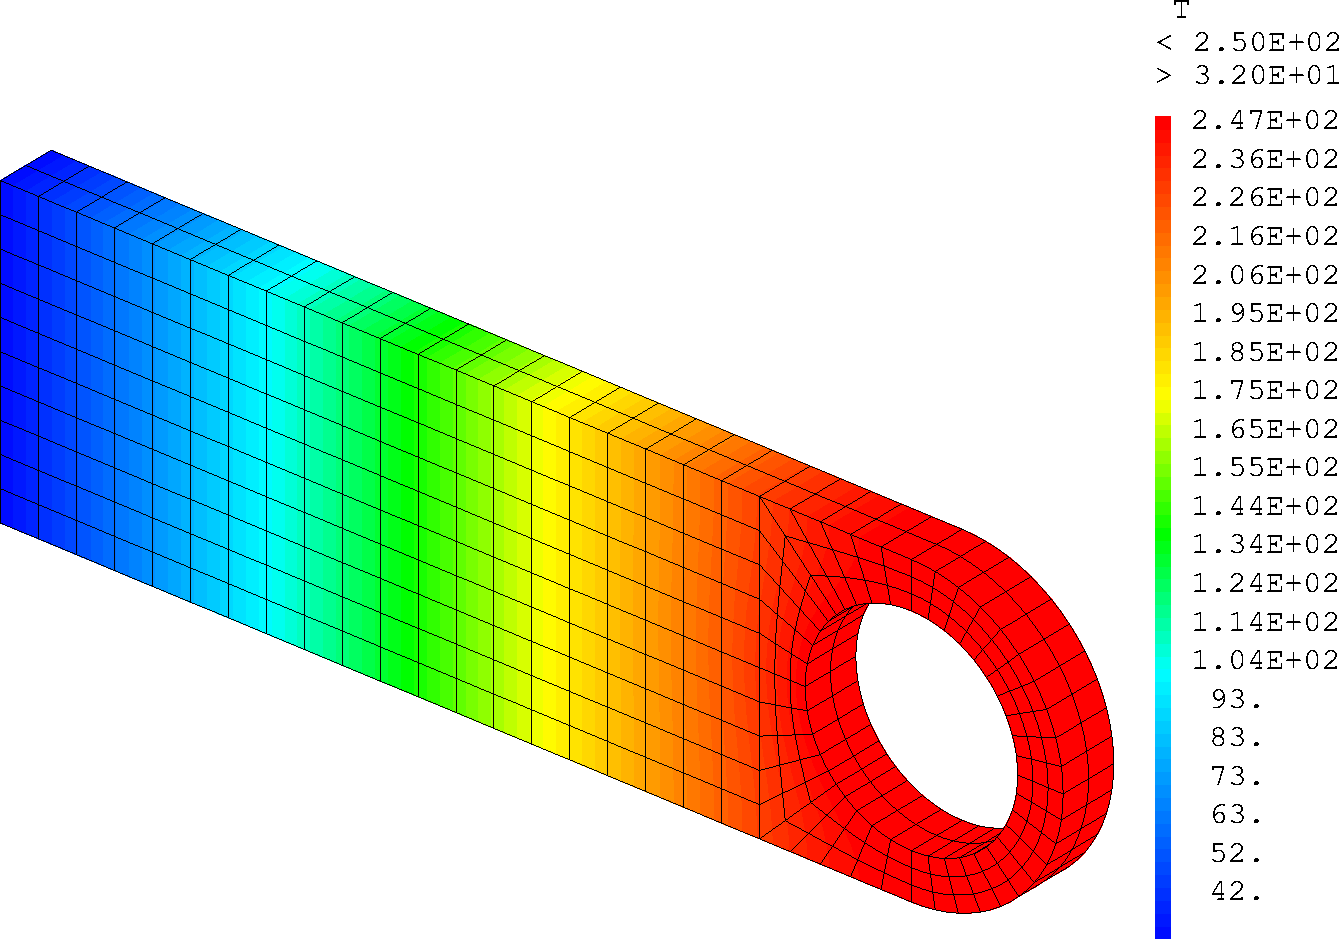
\includegraphics[height=0.5\textheight]{images/exo/2.1_temperatures.1}
      \end{textblock*}}
    \onslide<3>{
      \begin{textblock*}{5cm}(6cm,-4cm)
        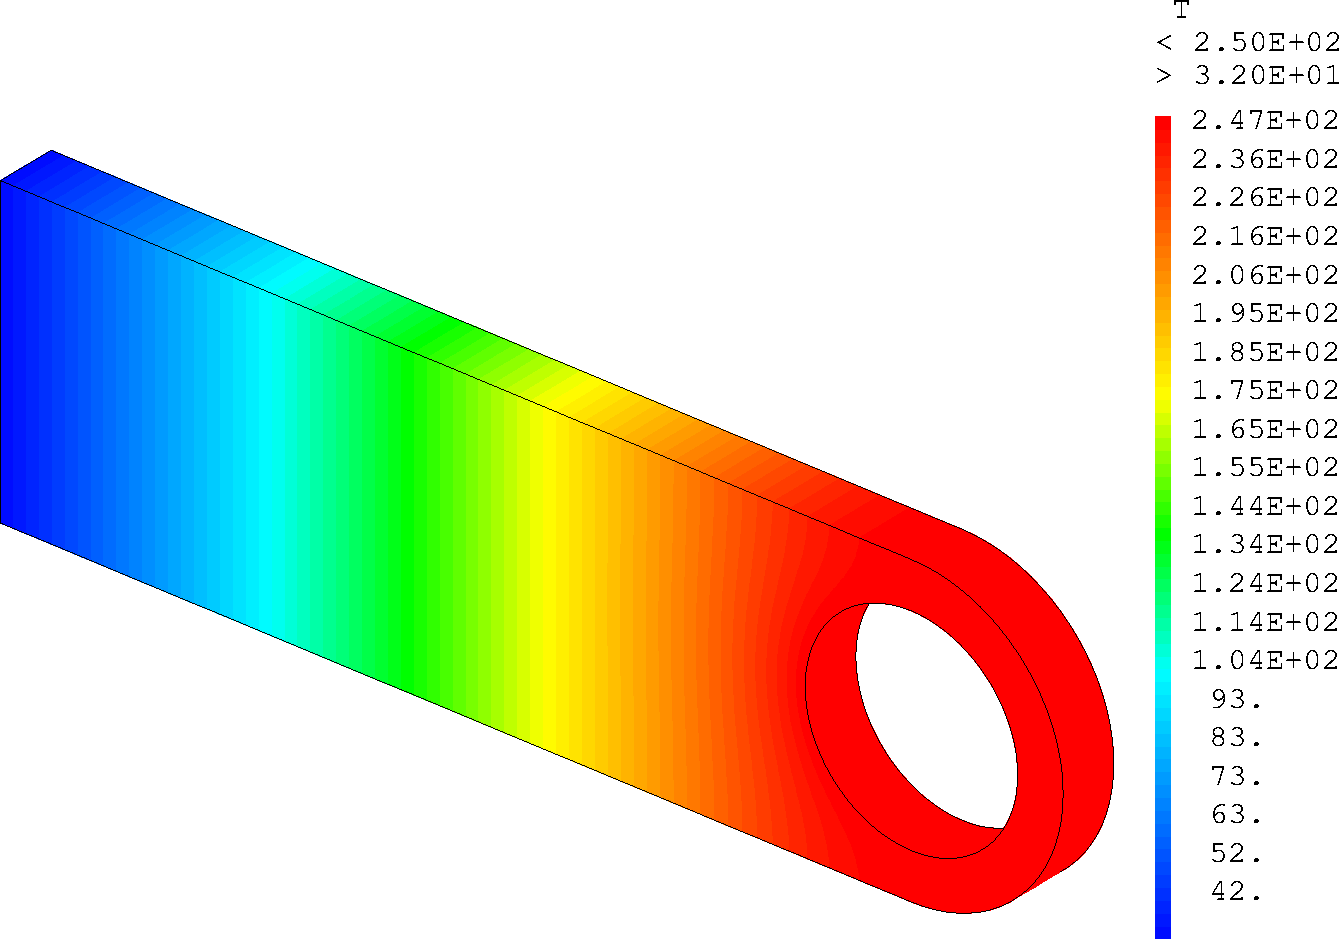
\includegraphics[height=0.5\textheight]{images/exo/2.1_temperatures.2}
      \end{textblock*}}
    \onslide<4>{
      \begin{textblock*}{5cm}(6cm,-4cm)
        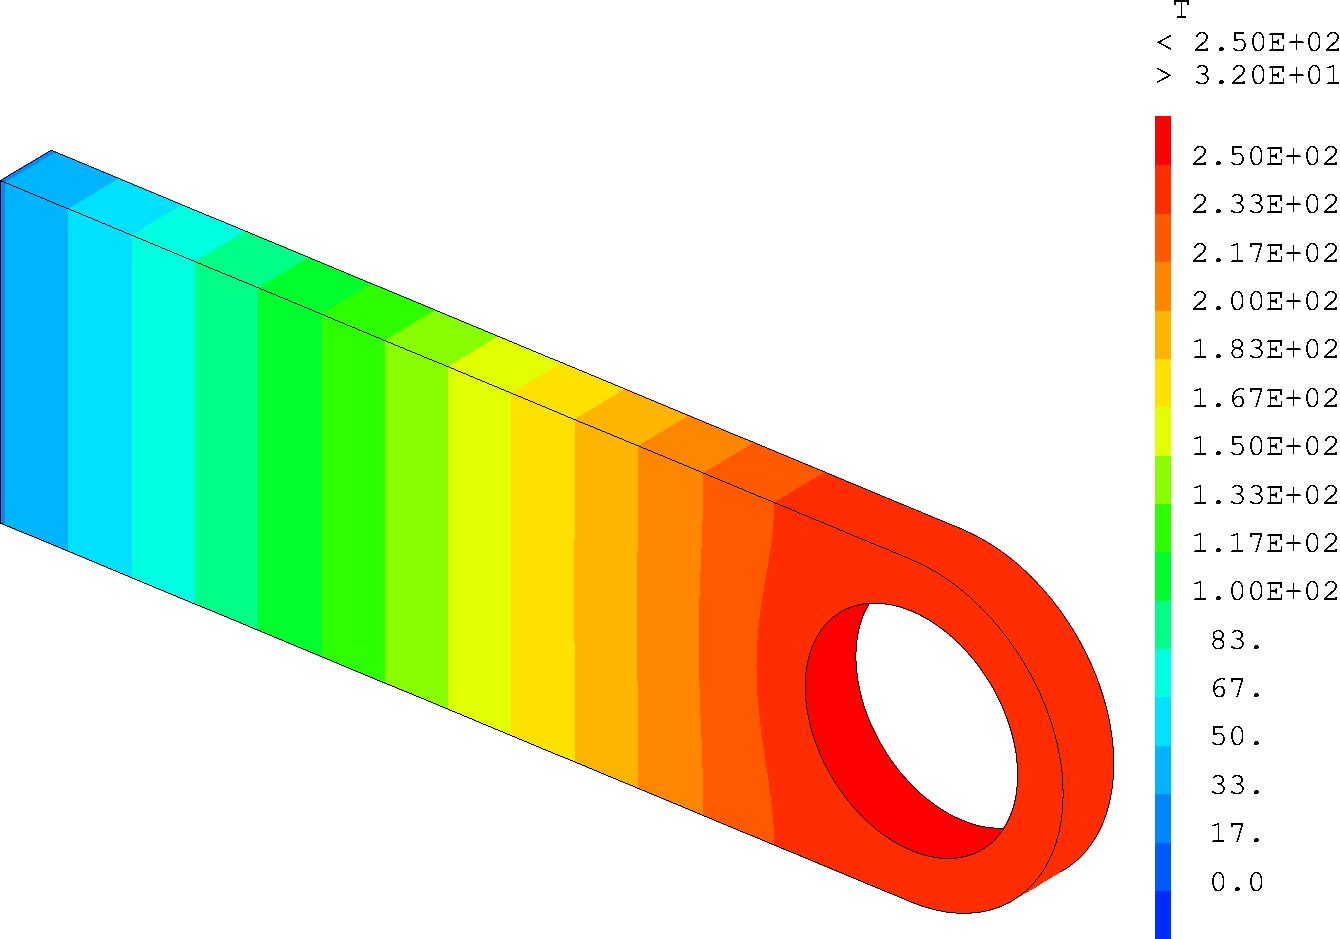
\includegraphics[height=0.5\textheight]{images/exo/2.1_temperatures.3}
      \end{textblock*}}
    \item[]<4> \violet{\emph{\fe{Nouvel objet :}{New object:} LISTREEL}}
  \end{itemize}
\end{frame}

\begin{frame}{\fe{2.2 Problème étudié}{2.2 Problem description}}
  \begin{itemize}
    \item \gray{\fe{Conduction, régime stationaire}{Conduction, steady state}}
    \begin{columns}
      \begin{column}{.4\textwidth}
        \item \gray{\fe{Température imposée}{Imposed temperature}}
        \footnotesize
        \begin{tikzpicture}
          \node[anchor=south west,inner sep=0,opacity=0.3] (image) at (0,0)
          {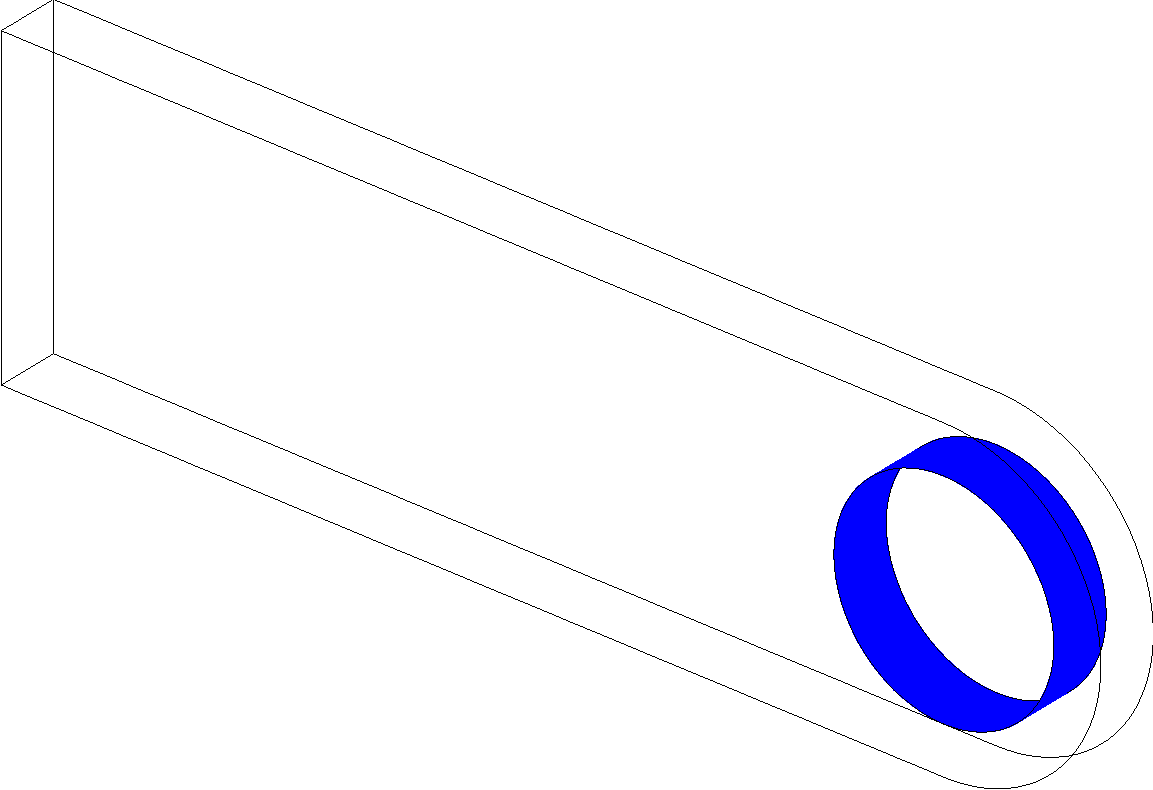
\includegraphics[width=3.5cm]{images/exo/2.1_cl_temperature}};
          \begin{scope}[x={(image.south east)},y={(image.north west)},color=blue,opacity=0.3]
            \draw (0.8,0.66) node[anchor=north west] {$T$~=~250~°C};
          \end{scope}
        \end{tikzpicture}
        \normalsize
      \end{column}
      \begin{column}{.4\textwidth}
        \item \gray{\fe{Flux de chaleur imposé}{Imposed heat flow}}
        \footnotesize
        \begin{tikzpicture}
          \node[anchor=south west,inner sep=0, opacity=0.3] (image) at (0,0)
          {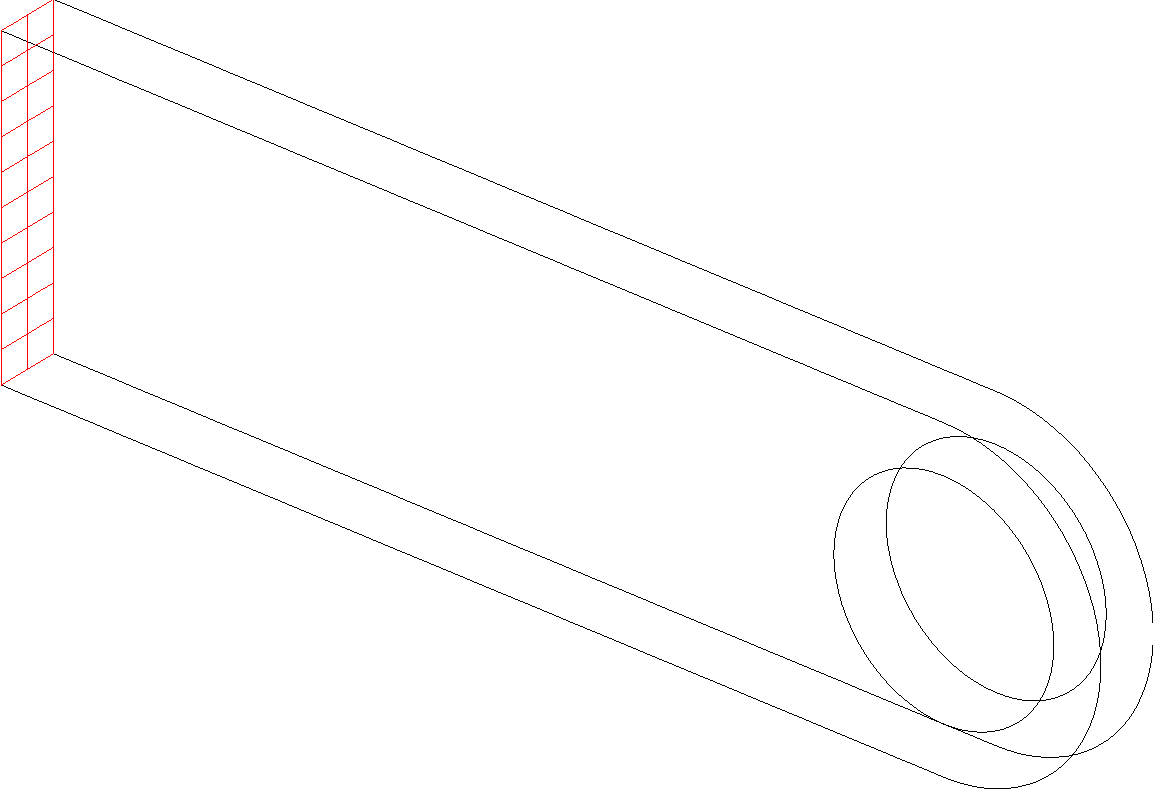
\includegraphics[width=3.5cm]{images/exo/2.1_cl_flux}};
          \begin{scope}[x={(image.south east)},y={(image.north west)},color=red,opacity=0.3]
            \draw (-0.25,0.5) node[anchor=north west,fill=white] {$\phi$~=~-40~kW.m$^{-2}$};
          \end{scope}
        \end{tikzpicture}
        \normalsize
      \end{column}
    \end{columns}
    \begin{columns}
      \begin{column}{.4\textwidth}
        \item \fe{\ul{Convection}}{\ul{Convection}}
        \footnotesize
        \begin{tikzpicture}
          \node[anchor=south west,inner sep=0] (image) at (0,0)
          {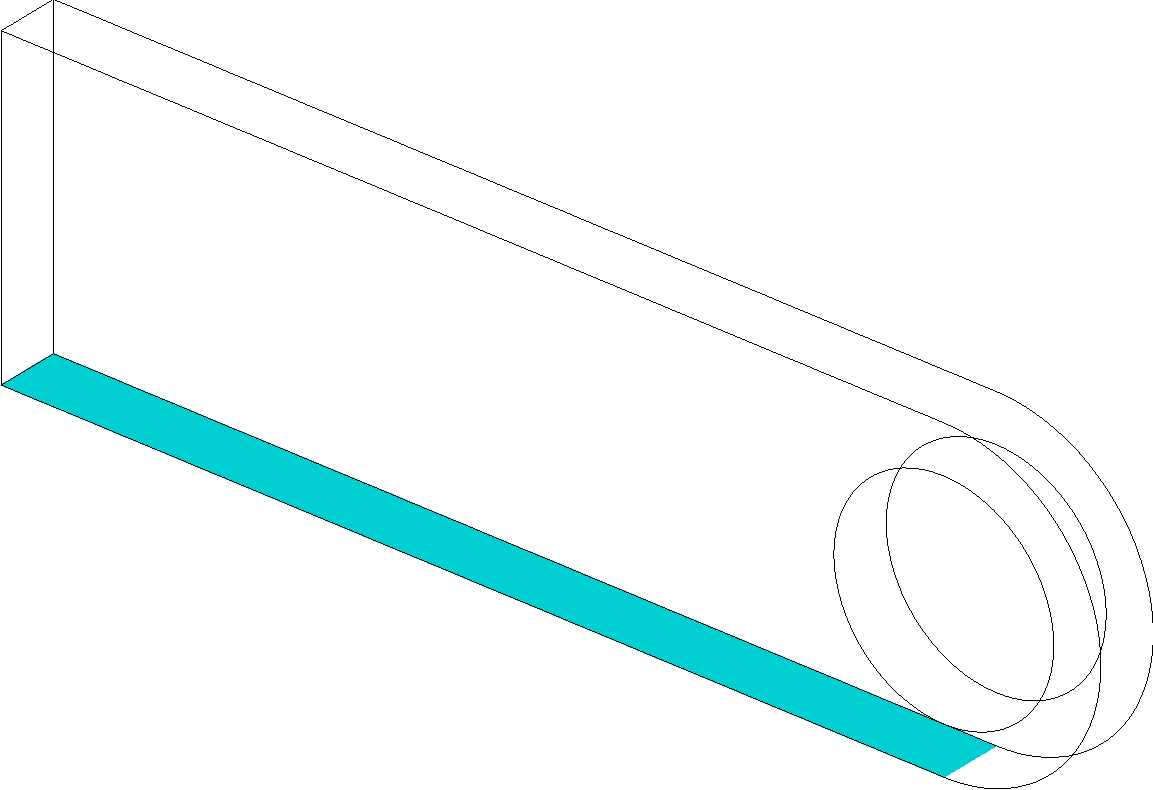
\includegraphics[width=3.5cm]{images/exo/2.2_cl_convection}};
          \begin{scope}[x={(image.south east)},y={(image.north west)},color=Aquamarine]
            \draw (-0.1,0.17) node[anchor=north west] {$T_f$~=~-80~°C};
            \draw (-0.1,0.07) node[anchor=north west] {$h$~=~240~W.m$^{-2}$.K$^{-1}$};
          \end{scope}
        \end{tikzpicture}
        \normalsize
      \end{column}
      \begin{column}{.4\textwidth}
        \item \fe{\ul{Source volumique}}{\ul{Volume source}}
        \footnotesize
        \begin{tikzpicture}
          \node[anchor=south west,inner sep=0] (image) at (0,0)
          {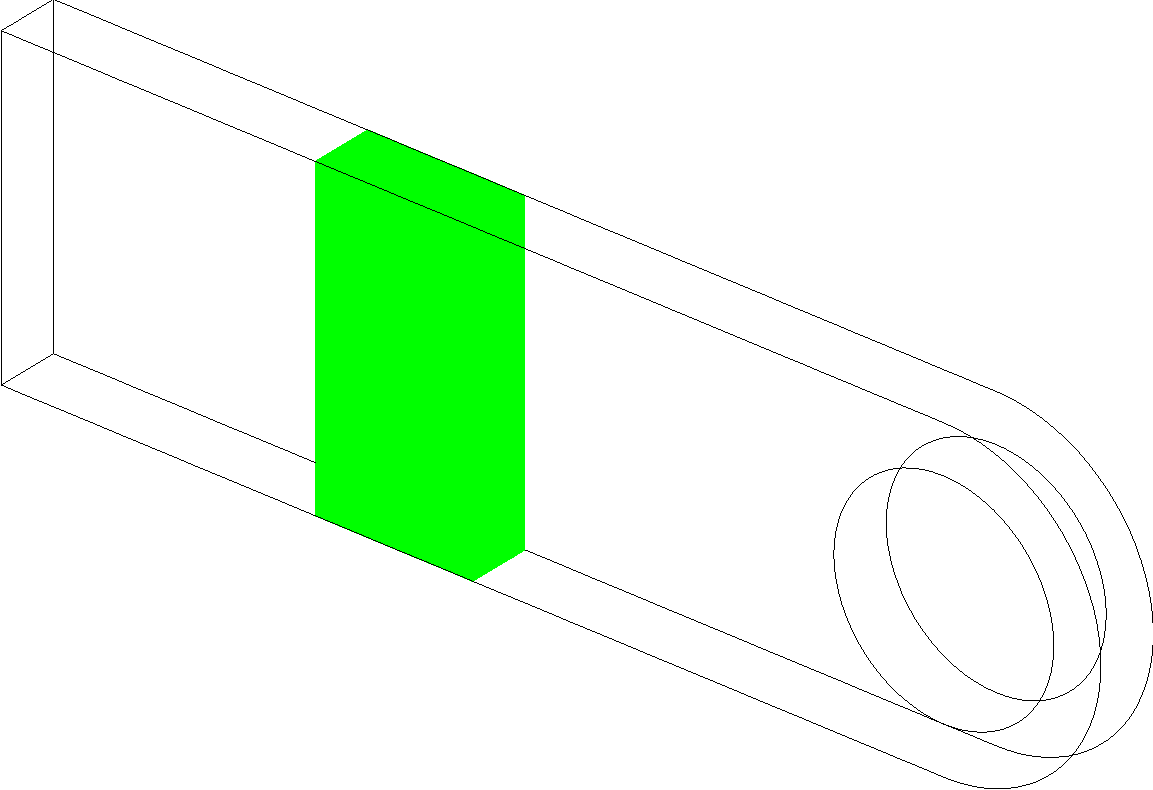
\includegraphics[width=3.5cm]{images/exo/2.2_cl_source}};
          \begin{scope}[x={(image.south east)},y={(image.north west)},color=green]
            \draw (0.5,0.7) node[anchor=south west] {$q$~=~2600~kW.m$^{-3}$};
          \end{scope}
        \end{tikzpicture}
        \normalsize
      \end{column}
    \end{columns}
  \end{itemize}
\end{frame}

\begin{frame}{\fe{2.2 Thermique linéaire}{2.2 Linear thermal analysis}}
             {\fe{Stationnaire, conduction, convection, source}{Steady state, conduction, convection, source}}
  \begin{itemize}
    \item \fe{Nouveaux paramètres}{New parameters}
    \lstinputlisting[language=gibiane, firstline=54, lastline=56]{dgibi/formation_debutant_2_thermique.dgibi}
    \item<2->\fe{Récupération de sous zones}{Subzone recovery}
    \onslide<2->{
      \lstinputlisting[language=gibiane, firstline=161, lastline=165]{dgibi/formation_debutant_2_thermique.dgibi}
      \lstinputlisting[language=gibiane, firstline=170, lastline=170]{dgibi/formation_debutant_2_thermique.dgibi}
      \begin{textblock*}{5cm}(8.6cm,-2.6cm)
        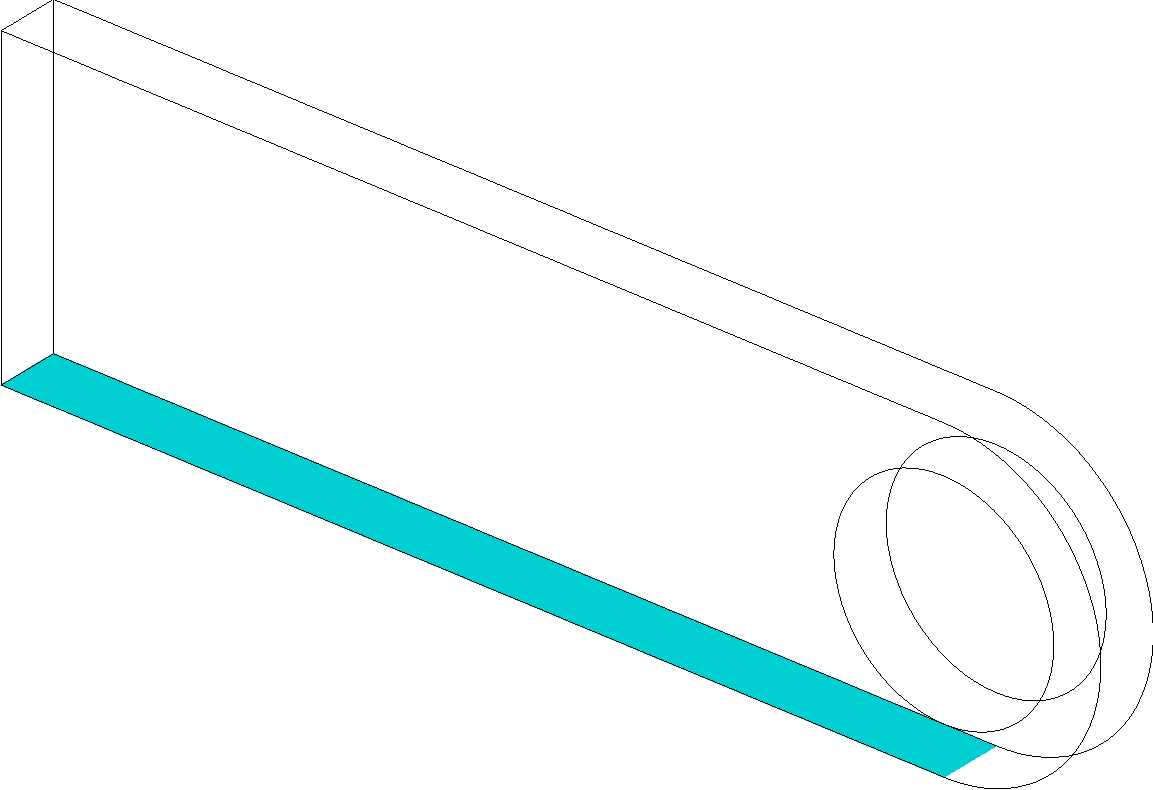
\includegraphics[width=3.5cm]{images/exo/2.2_cl_convection}
      \end{textblock*}}
    \onslide<3->{
      \lstinputlisting[language=gibiane, firstline=146, lastline=150]{dgibi/formation_debutant_2_thermique.dgibi}
      \lstinputlisting[language=gibiane, firstline=155, lastline=155]{dgibi/formation_debutant_2_thermique.dgibi}
      \begin{textblock*}{5cm}(8.6cm,-2.6cm)
        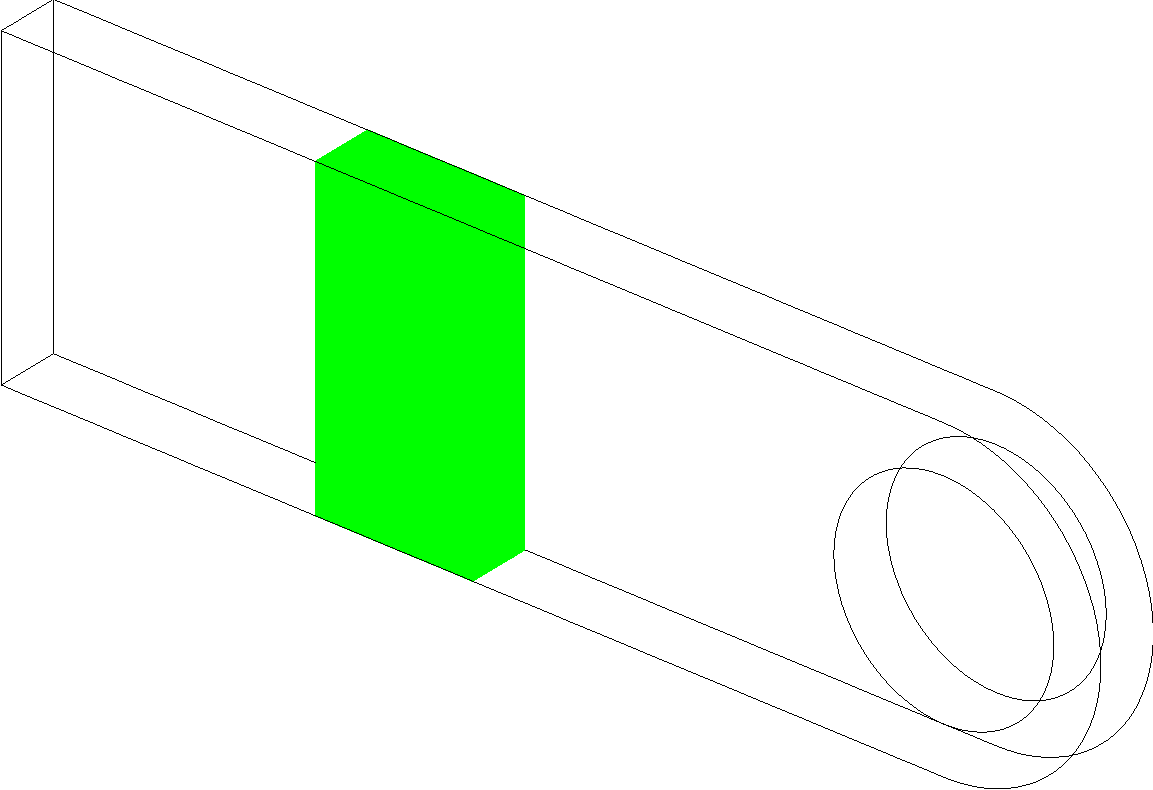
\includegraphics[width=3.5cm]{images/exo/2.2_cl_source}
      \end{textblock*}}
    \end{itemize}
\end{frame}

\begin{frame}{\fe{2.2 Thermique linéaire}{2.2 Linear thermal analysis}}
             {\fe{Stationnaire, conduction, convection, source}{Steady state, conduction, convection, source}}
  \begin{itemize}
    \item \fe{Formulation mathématique (convection)}{Mathematical formulation (convection)}
    \lstinputlisting[language=gibiane, firstline=173, lastline=175]{dgibi/formation_debutant_2_thermique.dgibi}
    \item<2->\fe{Matrice de conductivité (mais pour la convection !)}
                {Conductivity matrix (but for convection!)}
    \onslide<2->{
      \lstinputlisting[language=gibiane, firstline=177, lastline=179]{dgibi/formation_debutant_2_thermique.dgibi}
      \begin{flushright}
        \footnotesize
        $[K]=\gray{\int_V[B]^T[\lambda][B]dV+}\int_{\partial V_{\phi}}h[N]^T[N]dS$
        \normalsize
      \end{flushright}}
    \item<3->\fe{Chargement nodal équivalent (convection)}
                {Equivalent nodal load (convection)}
    \onslide<3->{
      \lstinputlisting[language=gibiane, firstline=181, lastline=184]{dgibi/formation_debutant_2_thermique.dgibi}
      \begin{flushright}
        \footnotesize
        $\{P\}=\gray{\int_V[N]^TqdV}+\int_{\partial V_{\phi}}[N]^T(\gray{\phi_{\tx{imp}}}+hT_f\gray{+\varepsilon\sigma(T_\infty^4-T^4)})dS$
        \normalsize
      \end{flushright}}
  \end{itemize}
\end{frame}

\begin{frame}{\fe{2.2 Thermique linéaire}{2.2 Linear thermal analysis}}
             {\fe{Stationnaire, conduction, convection, source}{Steady state, conduction, convection, source}}
  \begin{itemize}
    \item \fe{Chargement nodal équivalent (source)}{Equivalent nodal load (source)}
    \lstinputlisting[language=gibiane, firstline=158, lastline=159]{dgibi/formation_debutant_2_thermique.dgibi}
    \begin{flushright}
      \footnotesize
      $\{P\}=\int_V[N]^TqdV\gray{+\int_{\partial V_{\phi}}[N]^T(\gray{\phi_{\tx{imp}}+}hT_f\gray{+\varepsilon\sigma(T_\infty^4-T^4)})dS}$
      \normalsize
    \end{flushright}
    \item<2->\fe{Résolution et affichage des résultats}{Solving and plotting results}
    \onslide<2->{\lstinputlisting[language=gibiane, firstline=186, lastline=187]{dgibi/formation_debutant_2_thermique.dgibi}}
    \onslide<2->{\lstinputlisting[language=gibiane, firstline=194, lastline=194]{dgibi/formation_debutant_2_thermique.dgibi}}
    \vspace{3cm}
    \onslide<2->{
      \begin{textblock*}{6cm}(6cm,-3.5cm)
        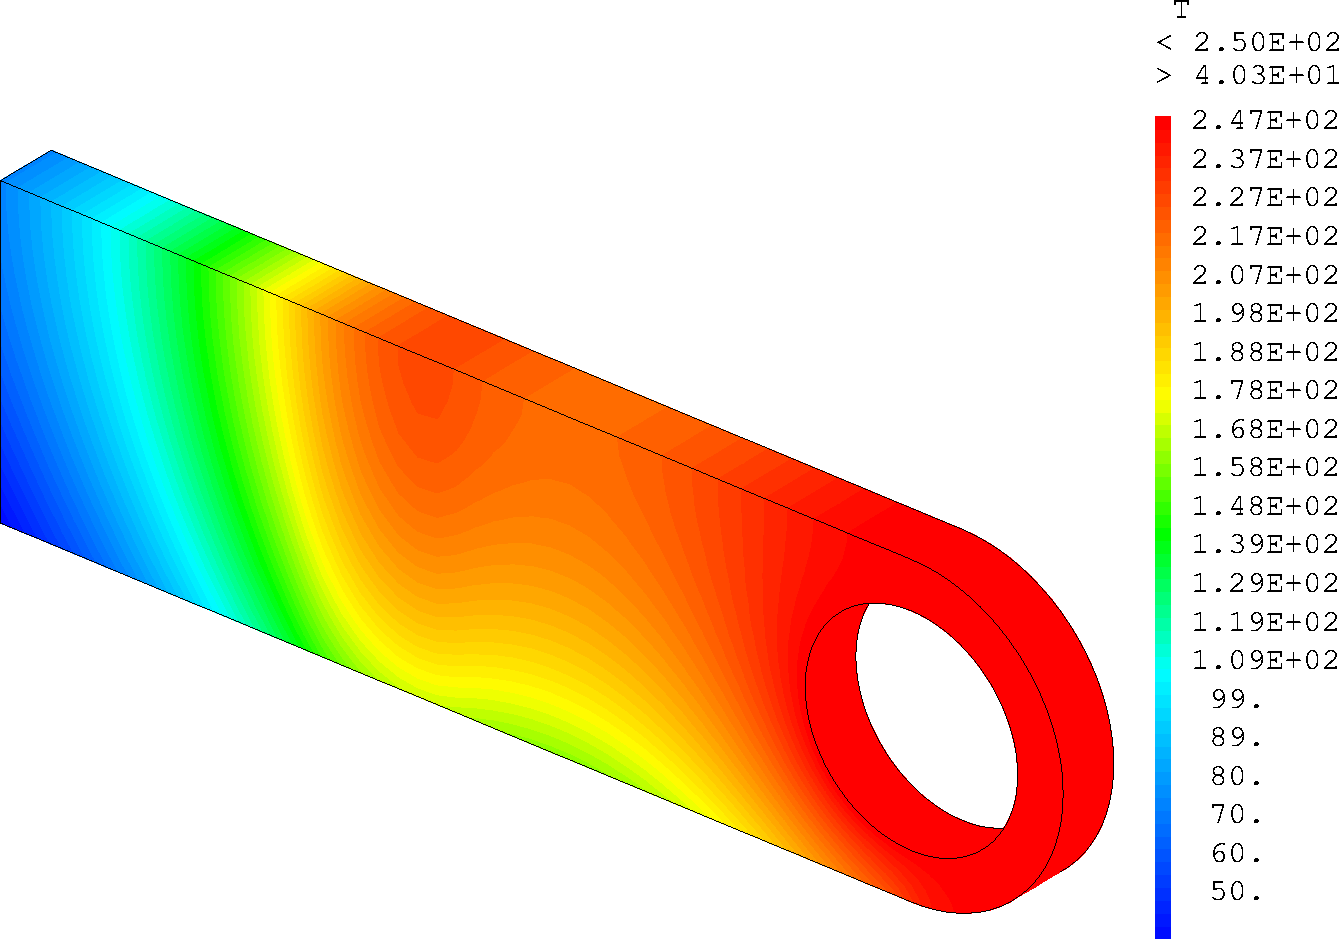
\includegraphics[height=0.4\textheight]{images/exo/2.2_temperatures}
      \end{textblock*}}
  \end{itemize}
\end{frame}

\begin{frame}{\fe{Remarques : champs par éléments (MCHAML)}
                 {Note: element fields (MCHAML)}}
  \begin{itemize}
    \item \fe{Objet MCHAML}{MCHAML object}\\
    \footnotesize
    \fe{Représente un champ de valeurs exprimées \g{dans les ÉLÉMENTS} d'un maillage}
       {Represents a field of values expressed \g{inside the ELEMENTS} of a mesh}\\
    \fe{Exemples :}{Examples:}
    \begin{textblock*}{6cm}(8.5cm,-0.3cm)
      \begin{tikzpicture}
        \node[anchor=south west,inner sep=0] (image) at (0,0)
        {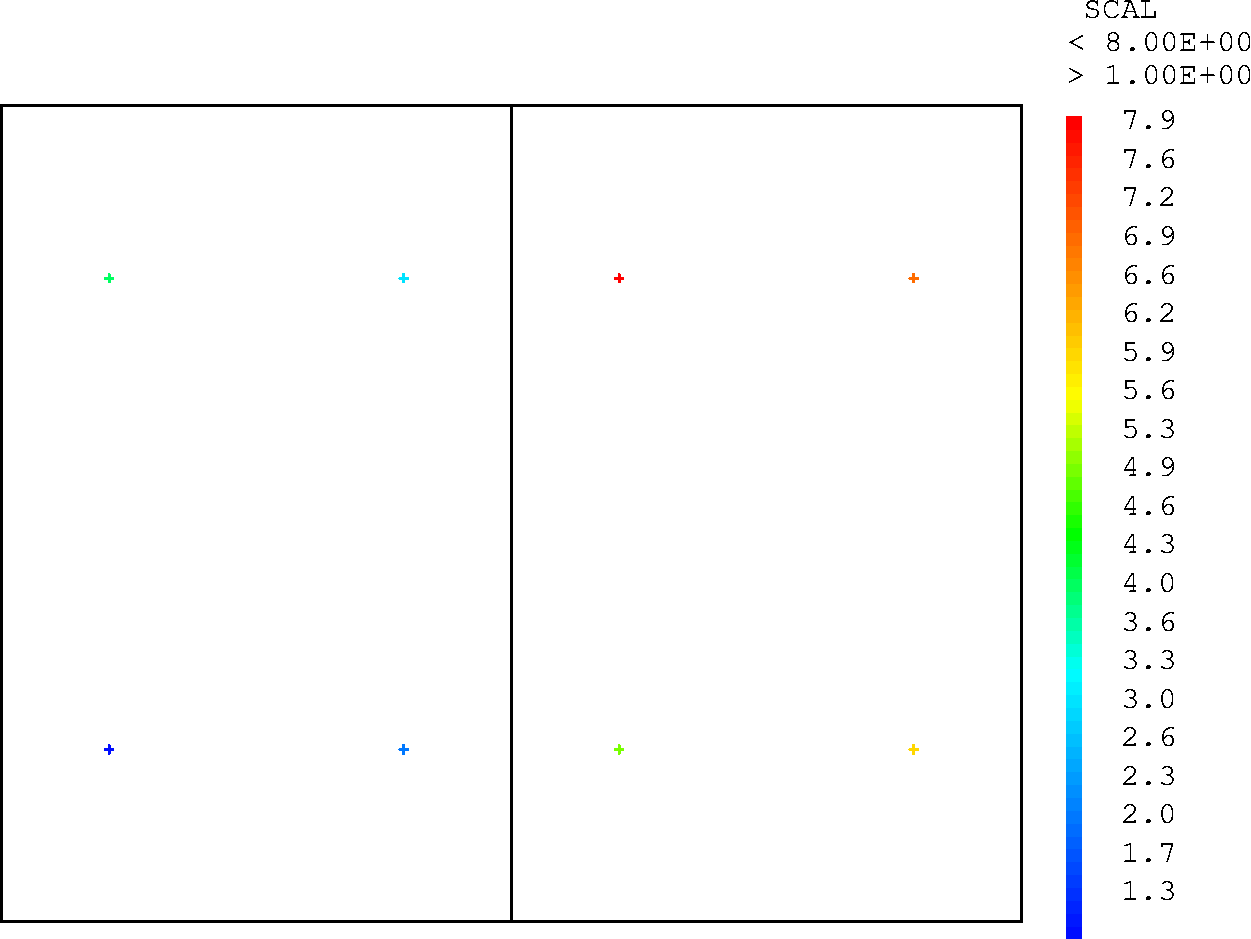
\includegraphics[width=3.8cm]{images/mchaml_chpoint.2}};
        \tiny
        \begin{scope}[x={(image.south east)},y={(image.north west)}]
          \draw (0.10,0.2) node[anchor=west] {1};
          \draw (0.32,0.2) node[anchor=east] {2};
          \draw (0.32,0.7) node[anchor=east] {3};
          \draw (0.10,0.7) node[anchor=west] {4};
          \draw (0.50,0.2) node[anchor=west] {5};
          \draw (0.73,0.2) node[anchor=east] {6};
          \draw (0.73,0.7) node[anchor=east] {7};
          \draw (0.50,0.7) node[anchor=west] {8};
        \end{scope}
      \end{tikzpicture}
    \end{textblock*}
    \begin{itemize}
      \footnotesize
      \item \fe{paramètres matériau}{material properties}
      \item \fe{gradient de températures, déplacements…}{gradient of temperatures, displacements…}
      \item \fe{contraintes, déformations}{stress, strains fields}
      \item \fe{variables internes}{internal variables field}
      \item \fe{et bien d'autres…}{and others…}
    \end{itemize}
    \footnotesize
    \fe{Quelques caractéristiques :}{Some characteristics:}
    \begin{textblock*}{6cm}(8.5cm,0.3cm)
      \begin{tikzpicture}
        \node[anchor=south west,inner sep=0] (image) at (0,0)
        {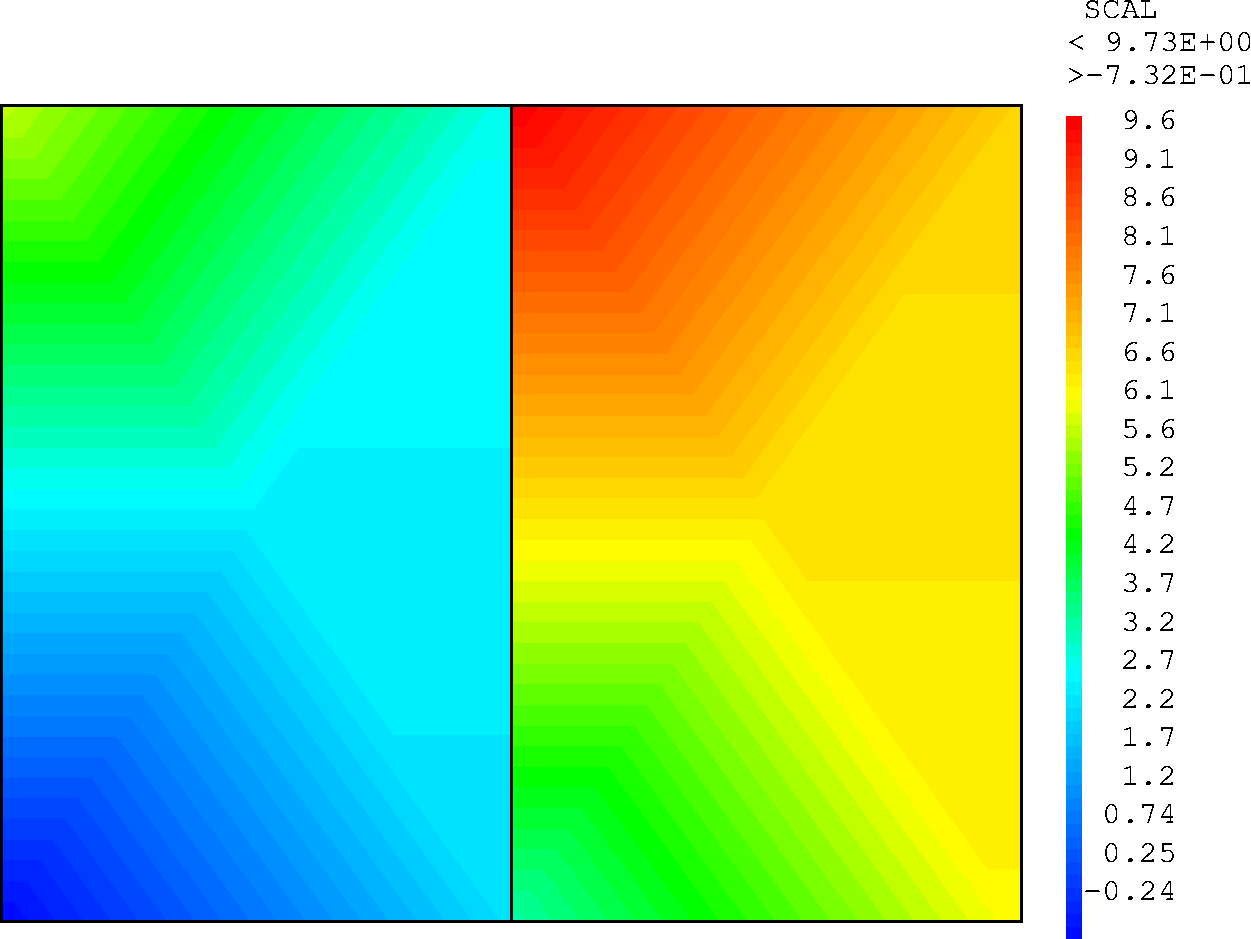
\includegraphics[width=3.8cm]{images/mchaml_chpoint.1}};
        \tiny
        \begin{scope}[x={(image.south east)},y={(image.north west)}]
          \draw (0.10,0.2) node[anchor=west] {1};
          \draw (0.32,0.2) node[anchor=east] {2};
          \draw (0.32,0.7) node[anchor=east] {3};
          \draw (0.10,0.7) node[anchor=west] {4};
          \draw (0.50,0.2) node[anchor=west] {5};
          \draw (0.73,0.2) node[anchor=east] {6};
          \draw (0.73,0.7) node[anchor=east] {7};
          \draw (0.50,0.7) node[anchor=west] {8};
        \end{scope}
      \end{tikzpicture}
    \end{textblock*}
    \begin{itemize}
      \footnotesize
      \item \fe{plusieurs points support possibles :}{several support points available:}\\
      \scriptsize
      ~\fe{points d'intégration des contraintes}{integration points for stresses}\\
      ~\fe{point d'intégration de la rigidité}{integration points for stiffness}\\
      ~\fe{points d'intégration de la masse}{integration points for mass}\\
      ~\fe{centre de gravité}{center of gravity}\\
      ~\fe{nœuds}{nodes}
      \footnotesize
      \item \fe{interpolé par les fonctions $[N(x)]$}{interpolation by $[N(x)]$ functions}
      \item \fe{non continu d'un élément à l'autre}{non continuous between elements}
    \end{itemize}
    \normalsize
  \end{itemize}
\end{frame}

\begin{frame}{\fe{Remarques : champs par points (CHPOINT)}
                 {Note: point fields (CHPOINT)}}
  \begin{itemize}
  \item \fe{Objet CHPOINT}{CHPOINT object}\\
    \footnotesize
    \fe{Représente un champ de valeurs exprimées sur des POINTS (nœuds)}
       {Respresents a field of values expressed \g{on POINTS (nodes)}}\\
    \fe{Exemples :}{Examples:}
    \begin{textblock*}{6cm}(8.5cm,-0.3cm)
      \begin{tikzpicture}
        \node[anchor=south west,inner sep=0] (image) at (0,0)
        {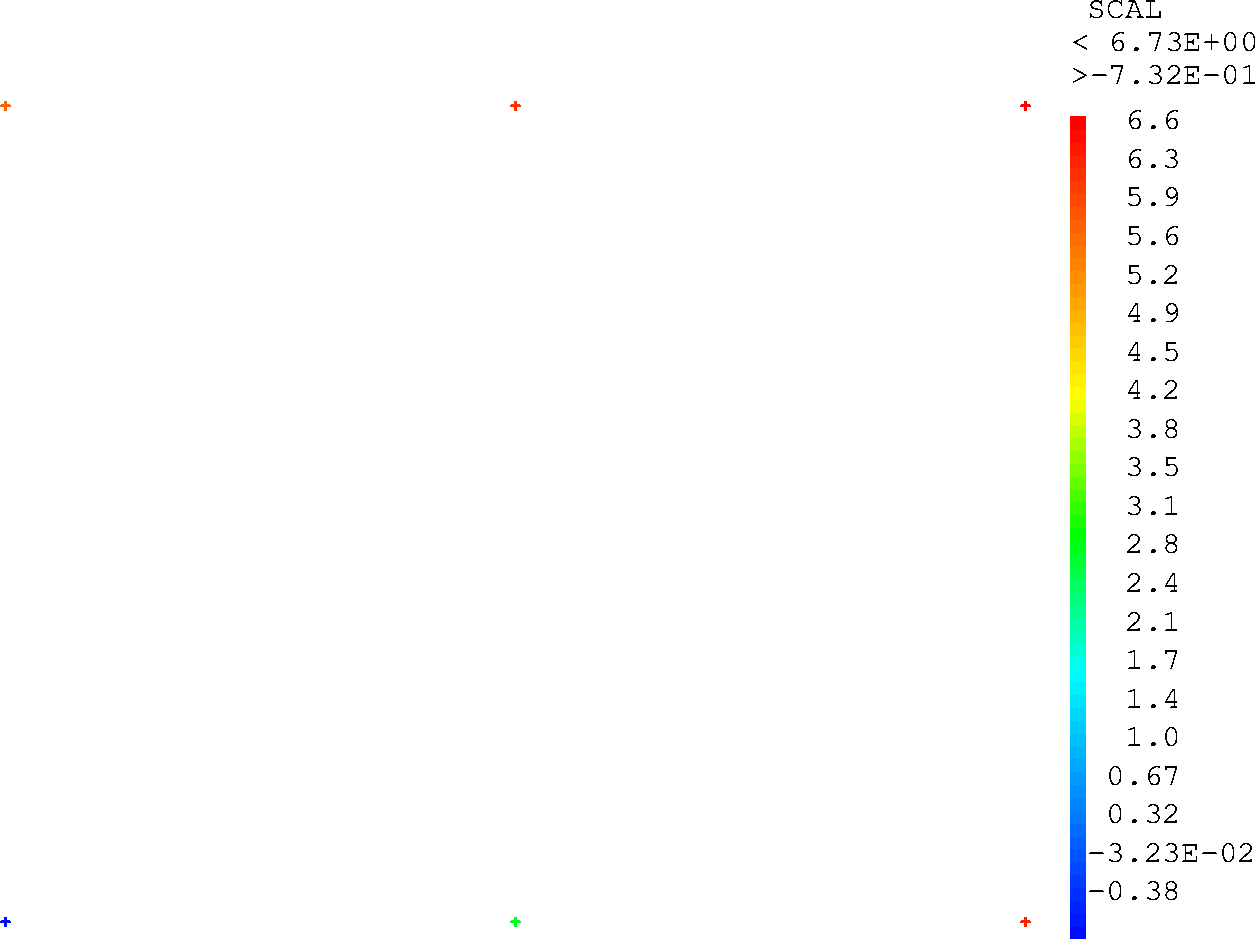
\includegraphics[width=3.8cm]{images/mchaml_chpoint.4}};
        \tiny
        \begin{scope}[x={(image.south east)},y={(image.north west)}]
          \draw (0,0)   node[anchor=south west] {-0.73};
          \draw (0.4,0) node[anchor=south west] {2.77};
          \draw (0.8,0) node[anchor=south east] {6.27};
          \draw (0,0.9) node[anchor=north west] {5.73};
          \draw (0.4,0.9) node[anchor=north west] {6.23};
          \draw (0.8,0.9) node[anchor=north east] {6.73};
        \end{scope}
      \end{tikzpicture}
    \end{textblock*}
    \begin{itemize}
      \footnotesize
      \item \fe{champ scalaire de température}{scalar temperature field}
      \item \fe{champ vectoriel de déplacement (3 composantes)}
               {vector displacement field (3 components)}
      \item \fe{champ vectoriel de coordonnées des nœuds}
               {vector coordinates fields}
      \item \fe{chargement nodal équivalent}{equivalent nodal load}
      \item \fe{et bien d'autres…}{and others…}
    \end{itemize}
    \footnotesize
    \fe{Quelques caractéristiques :}{Some characteristics:}
    \begin{textblock*}{6cm}(8.5cm,0.3cm)
      \begin{tikzpicture}
        \node[anchor=south west,inner sep=0] (image) at (0,0)
        {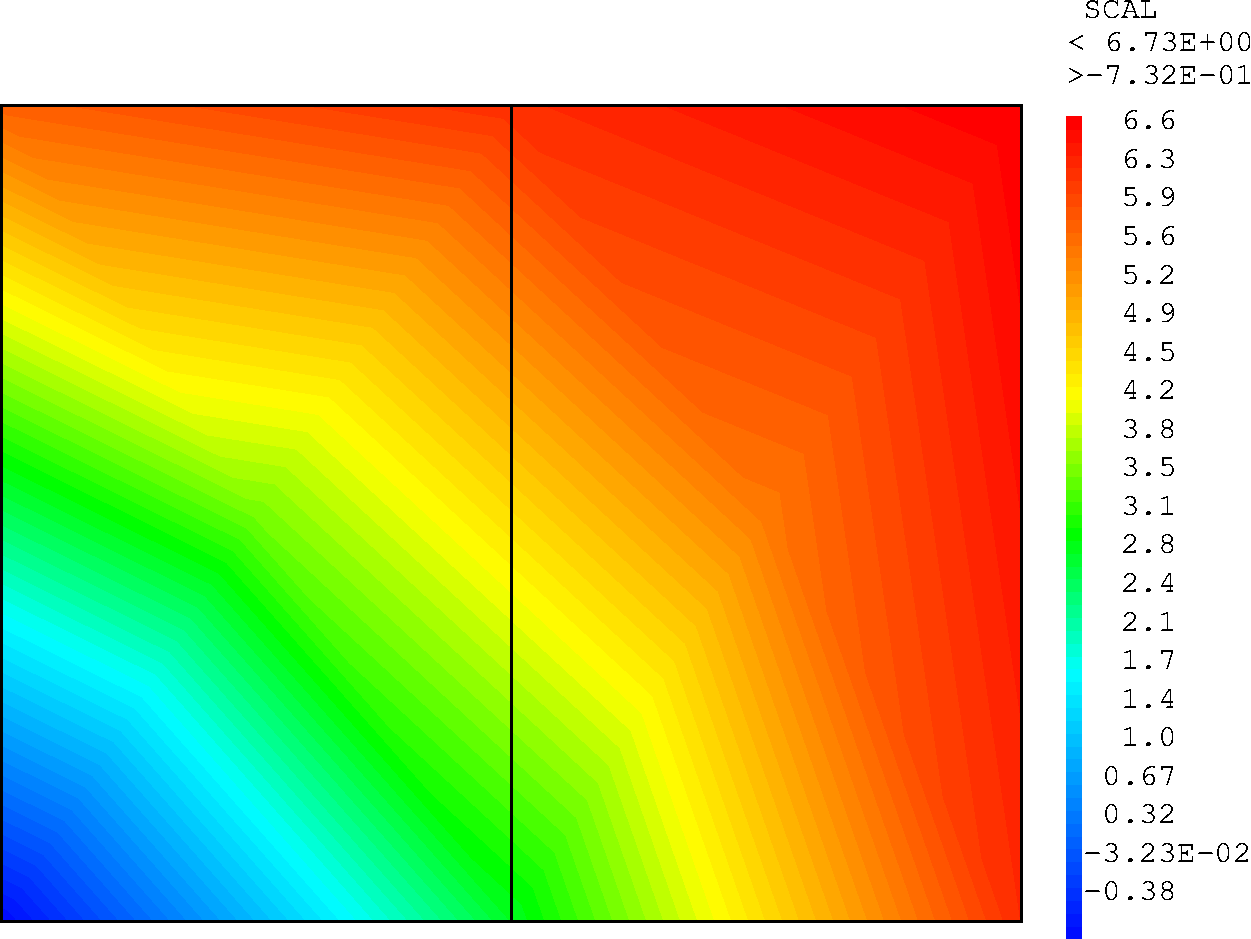
\includegraphics[width=3.8cm]{images/mchaml_chpoint.3}};
        \tiny
        \begin{scope}[x={(image.south east)},y={(image.north west)}]
          \draw (0,0)   node[anchor=south west] {-0.73};
          \draw (0.4,0) node[anchor=south west] {2.77};
          \draw (0.8,0) node[anchor=south east] {6.27};
          \draw (0,0.9) node[anchor=north west] {5.73};
          \draw (0.4,0.9) node[anchor=north west] {6.23};
          \draw (0.8,0.9) node[anchor=north east] {6.73};
        \end{scope}
      \end{tikzpicture}
    \end{textblock*}
    \begin{itemize}
      \footnotesize
      \item \fe{une seule valeur possible par nœud}{only one value per node}
      \item \fe{ne dépend pas du maillage,\\seulement des nœuds !}
               {do not depends on the mesh,\\ only on nodes!}
      \item \fe{continu sur le maillage}
               {continuous over the mesh}
    \end{itemize}
    \normalsize
  \end{itemize}
  \vspace{1.5cm}
\end{frame}

\begin{frame}{\fe{3 Problème étudié}{3 Problem description}}
  \begin{itemize}
    \item \fe{Conduction, \ul{régime transitoire}}{Conduction, \ul{transient}}
    \begin{columns}
      \begin{column}{.4\textwidth}
        \item \gray{\fe{Température imposée}{Imposed temperature}}
        \footnotesize
        \begin{tikzpicture}
          \node[anchor=south west,inner sep=0,opacity=0.3] (image) at (0,0)
          {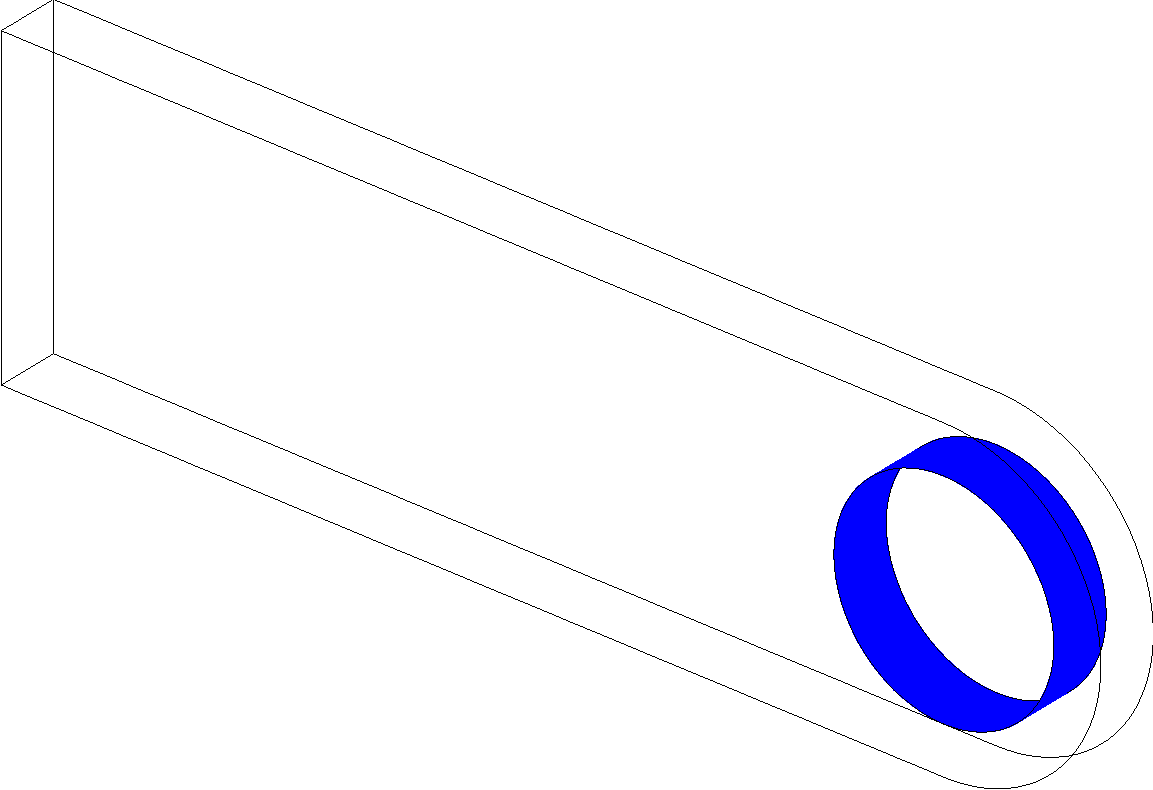
\includegraphics[width=3.5cm]{images/exo/2.1_cl_temperature}};
          \begin{scope}[x={(image.south east)},y={(image.north west)},color=blue,opacity=0.3]
            \draw (0.8,0.66) node[anchor=north west] {$T$~=~250~°C};
          \end{scope}
        \end{tikzpicture}
        \normalsize
      \end{column}
      \begin{column}{.4\textwidth}
        \item \gray{\fe{Flux de chaleur imposé}{Imposed heat flow}}
        \footnotesize
        \begin{tikzpicture}
          \node[anchor=south west,inner sep=0, opacity=0.3] (image) at (0,0)
          {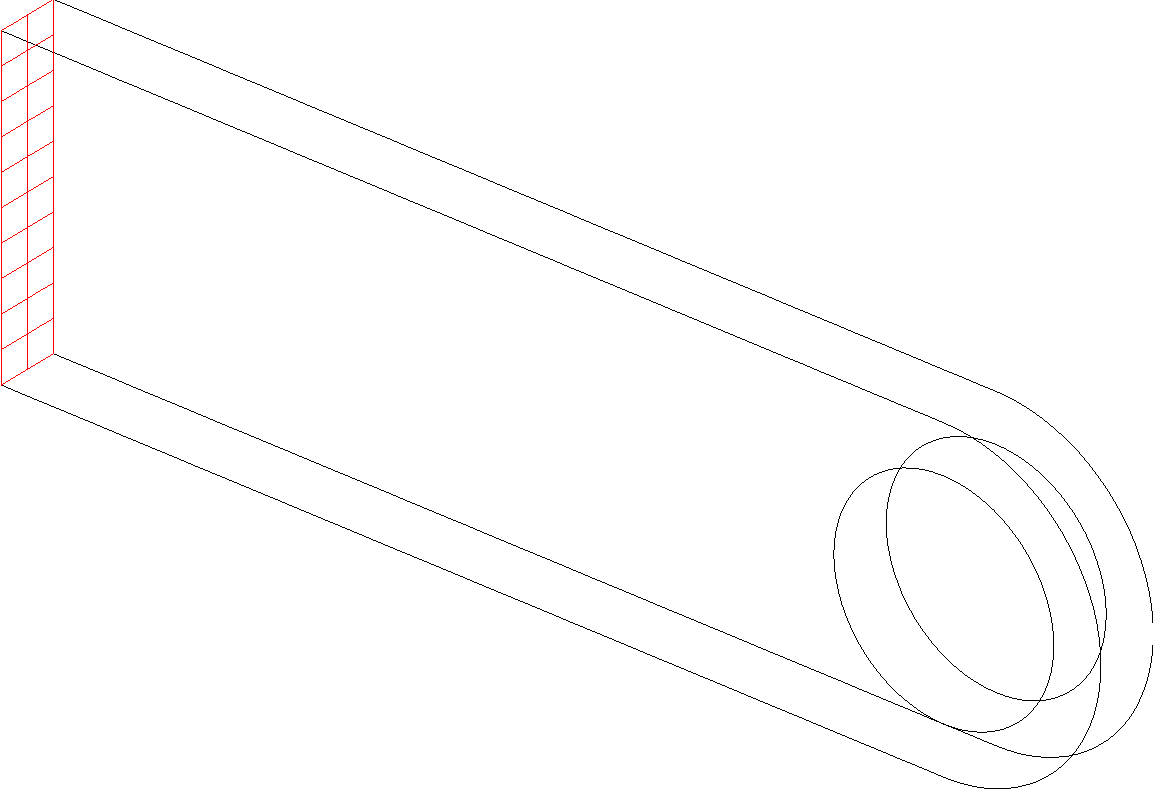
\includegraphics[width=3.5cm]{images/exo/2.1_cl_flux}};
          \begin{scope}[x={(image.south east)},y={(image.north west)},color=red,opacity=0.3]
            \draw (-0.25,0.5) node[anchor=north west,fill=white] {$\phi$~=~-40~kW.m$^{-2}$};
          \end{scope}
        \end{tikzpicture}
        \normalsize
      \end{column}
    \end{columns}
    \begin{columns}
      \begin{column}{.4\textwidth}
        \item \gray{Convection}
        \footnotesize
        \begin{tikzpicture}
          \node[anchor=south west,inner sep=0, opacity=0.3] (image) at (0,0)
          {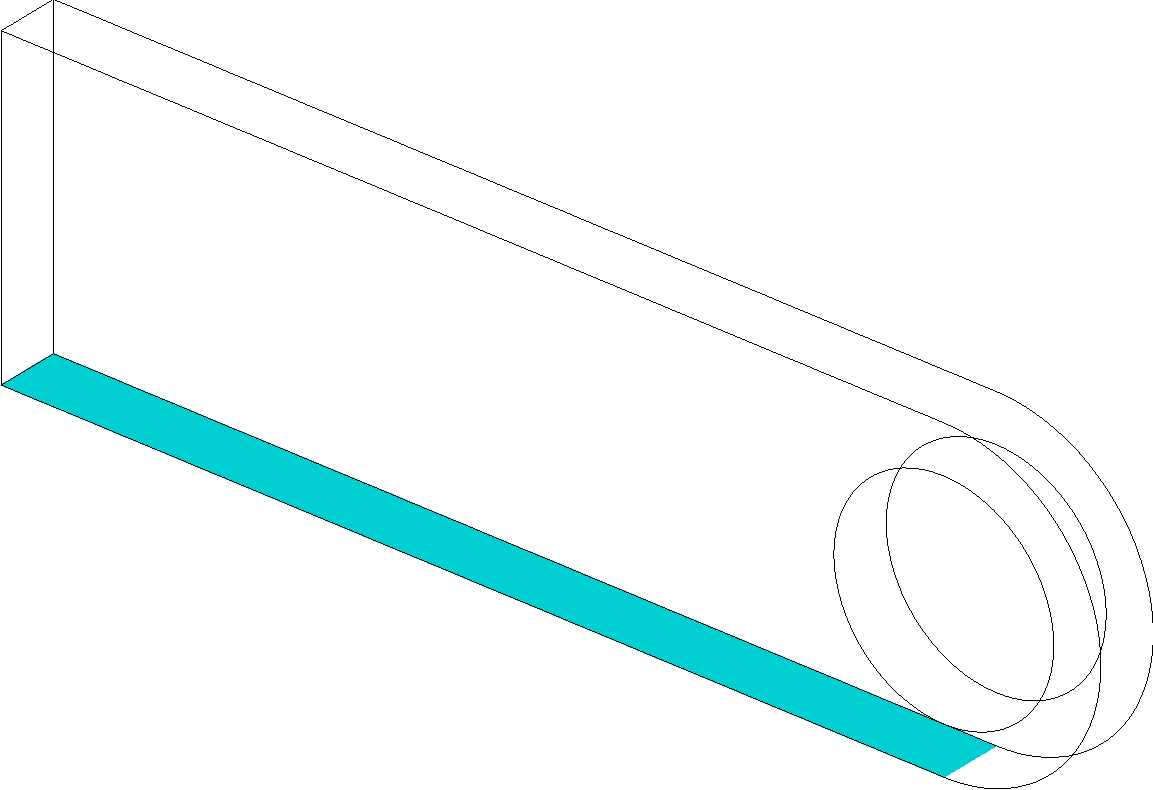
\includegraphics[width=3.5cm]{images/exo/2.2_cl_convection}};
          \begin{scope}[x={(image.south east)},y={(image.north west)},color=Aquamarine,opacity=0.3]
            \draw (-0.1,0.17) node[anchor=north west] {$T_f$~=~-80~°C};
            \draw (-0.1,0.07) node[anchor=north west] {$h$~=~240~W.m$^{-2}$.K$^{-1}$};
          \end{scope}
        \end{tikzpicture}
        \normalsize
      \end{column}
      \begin{column}{.4\textwidth}
        \item \gray{\fe{Source volumique}{Volume source}}
        \footnotesize
        \begin{tikzpicture}
          \node[anchor=south west,inner sep=0, opacity=0.3] (image) at (0,0)
          {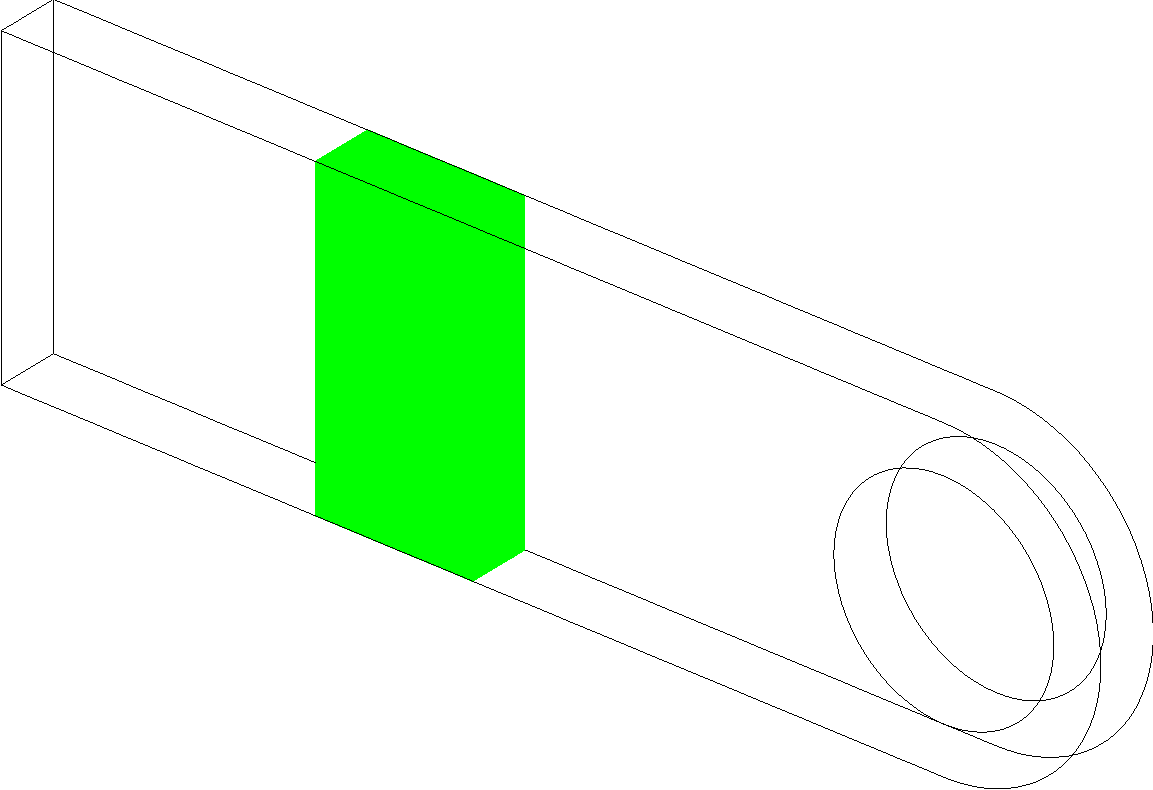
\includegraphics[width=3.5cm]{images/exo/2.2_cl_source}};
          \begin{scope}[x={(image.south east)},y={(image.north west)},color=green,opacity=0.3]
            \draw (0.5,0.7) node[anchor=south west] {$q$~=~2600~kW.m$^{-3}$};
          \end{scope}
        \end{tikzpicture}
        \normalsize
      \end{column}
    \end{columns}
  \end{itemize}
\end{frame}

\begin{frame}{\fe{3 Thermique linéaire}{3 Linear thermal analysis}}
             {\fe{Transitoire, conduction, convection, source}{Transient, conduction, convection, source}}
  \begin{itemize}
    \item \fe{Objectif : calcul thermique transitoire}{Objective: transient thermal calculation}
    \begin{center}
      $[C]\{\dot{T}\}+[K]\{T\}=\{P\}$
    \end{center}
    \item \fe{Méthode :}{Method:}\\
    \begin{tabular}{ll}
      \fe{description temporelle des chargements}{time description of loads}\\
      \fe{conditions initiales}{initial conditions}\\
      \fe{résolution avec la procédure \kwo{PASAPAS}}{using the \kwo{PASAPAS} solving procedure}\\
    \end{tabular}
  \end{itemize}
\end{frame}

\begin{frame}{\fe{3 Thermique linéaire}{3 Linear thermal analysis}}
             {\fe{Transitoire, conduction, convection, source}{Transient, conduction, convection, source}}
  \begin{itemize}
    \item \fe{Intervalle de temps}{Time interval }
    \lstinputlisting[basicstyle=\ttfamily\tiny, language=gibiane, firstline=60, lastline=61]{dgibi/formation_debutant_2_thermique.dgibi}
    \item<2->\fe{Chargements : description temporelle}{Loads: time description}
    \onslide<2->{
      \lstinputlisting[basicstyle=\ttfamily\tiny, language=gibiane, firstline=213, lastline=219]{dgibi/formation_debutant_2_thermique.dgibi}}
    \onslide<3->{
      \lstinputlisting[basicstyle=\ttfamily\tiny, language=gibiane, firstline=220, lastline=224]{dgibi/formation_debutant_2_thermique.dgibi}}
    \onslide<4->{
      \lstinputlisting[basicstyle=\ttfamily\tiny, language=gibiane, firstline=225, lastline=226]{dgibi/formation_debutant_2_thermique.dgibi}
      \lstinputlisting[basicstyle=\ttfamily\tiny, language=gibiane, firstline=227, lastline=228]{dgibi/formation_debutant_2_thermique.dgibi}}
    \item[]<2-> \violet{\emph{\fe{Nouveaux objets :}{New objects:} EVOLUTIOn, CHARGEMEnt}}
  \end{itemize}
\end{frame}

\begin{frame}{\fe{3 Thermique linéaire}{3 Linear thermal analysis}}
             {\fe{Transitoire, conduction, convection, source}{Transient, conduction, convection, source}}
  \begin{itemize}
    \item \fe{Construction d'une table pour \kwo{PASAPAS}}{Construction of a table for \kwo{PASAPAS}}
    \lstinputlisting[language=gibiane, firstline=230, lastline=239]{dgibi/formation_debutant_2_thermique.dgibi}
    \item<2->\fe{Résolution avec \kwo{PASAPAS}}{Solving with \kwo{PASAPAS}}
    \onslide<2->{
      \lstinputlisting[language=gibiane, firstline=240, lastline=240]{dgibi/formation_debutant_2_thermique.dgibi}}
    \item[]<1-> \violet{\emph{\fe{Nouvel objet :}{New object:} TABLE}}
  \end{itemize}
\end{frame}

\begin{frame}{\fe{3 Thermique linéaire}{3 Linear thermal analysis}}
             {\fe{Transitoire, conduction, convection, source}{Transient, conduction, convection, source}}
  \begin{itemize}
    \item \fe{Post traitement : évolutions temporelles}{Post processing: time curves}
    \lstinputlisting[basicstyle=\ttfamily\tiny, language=gibiane, firstline=242, lastline=248]{dgibi/formation_debutant_2_thermique.dgibi}
    \onslide<2->{
      \lstinputlisting[basicstyle=\ttfamily\tiny, language=gibiane, firstline=253, lastline=253]{dgibi/formation_debutant_2_thermique.dgibi}
      \begin{textblock*}{6cm}(8cm,-2.8cm)
        \begin{tikzpicture}
          \node[anchor=south west,inner sep=0] (image) at (0,0)
          {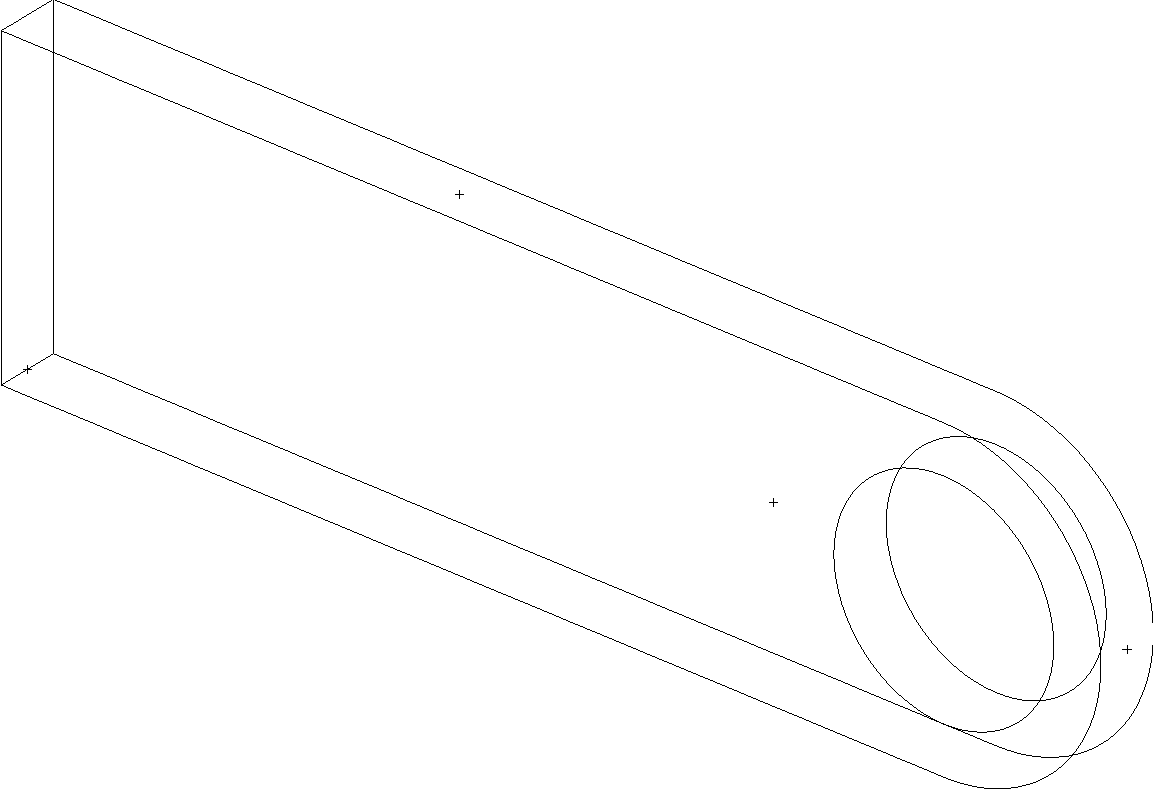
\includegraphics[width=4.2cm]{images/exo/3_points}};
          \begin{scope}[x={(image.south east)},y={(image.north west)}]
            \tiny
            \draw (0.02,0.51) node[anchor=west] {\kwb{pa}};
            \draw (0.4,0.75) node[anchor=west] {\kwg{pb}};
            \draw (0.67,0.36) node[anchor=east] {\kwo{pc}};
            \draw (0.99,0.18) node[anchor=west] {\kwr{pd}};
          \end{scope}
        \end{tikzpicture}
      \end{textblock*}}
    \onslide<3->{
      \lstinputlisting[basicstyle=\ttfamily\tiny, language=gibiane, firstline=255, lastline=258]{dgibi/formation_debutant_2_thermique.dgibi}
      \lstinputlisting[basicstyle=\ttfamily\tiny, language=gibiane, firstline=263, lastline=263]{dgibi/formation_debutant_2_thermique.dgibi}
      \begin{textblock*}{6cm}(6.5cm,-0.3cm)
        \begin{tikzpicture}
          \node[anchor=south west,inner sep=0] (image) at (0,0)
          {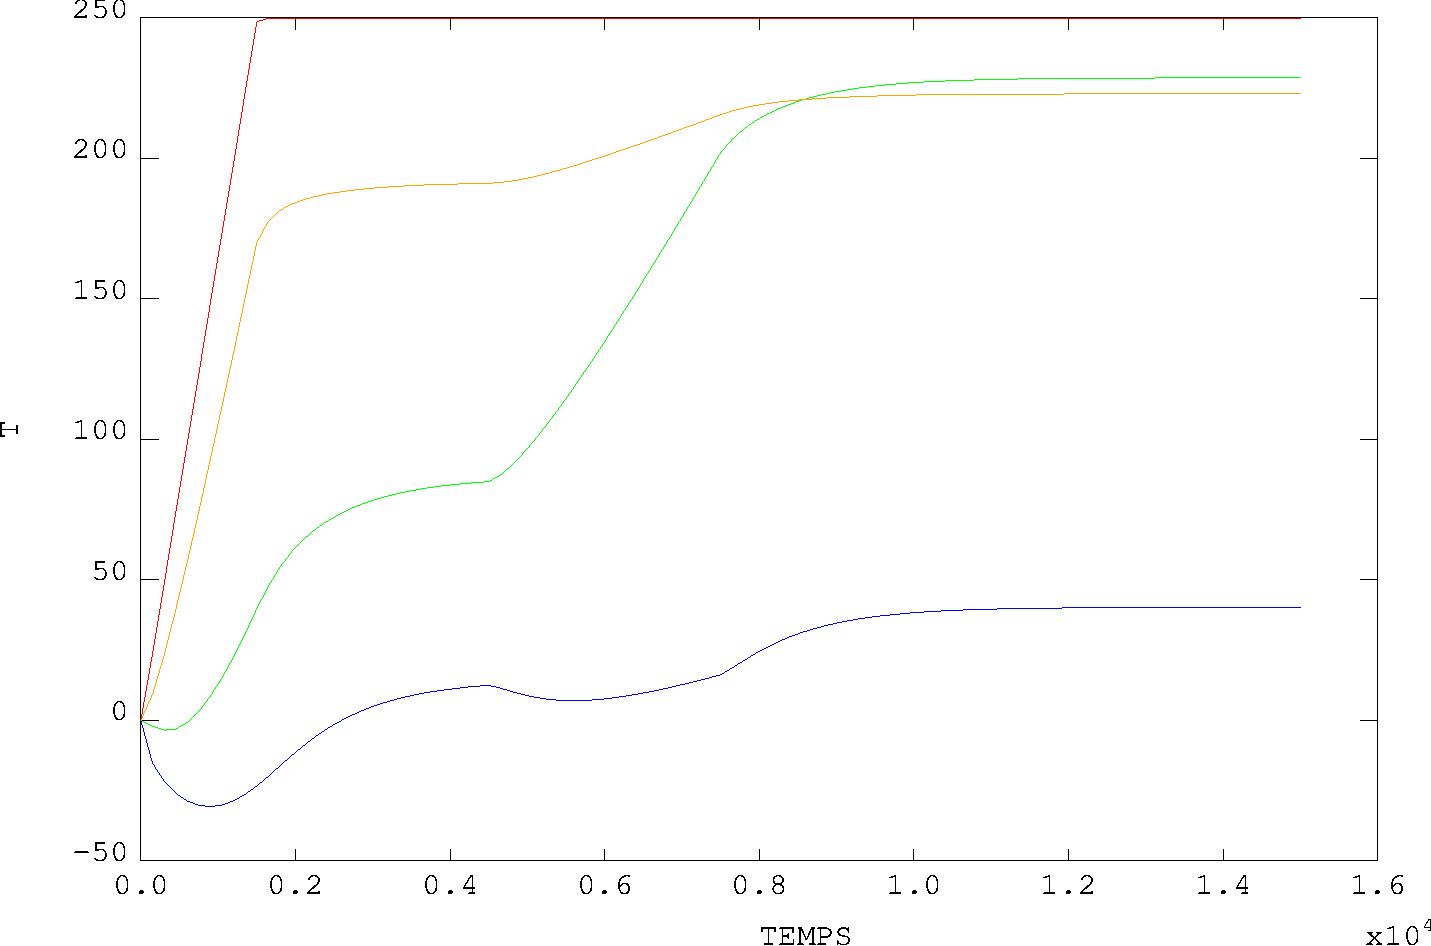
\includegraphics[width=4.8cm]{images/exo/3_evol_temperatures}};
        \end{tikzpicture}
      \end{textblock*}}
    \end{itemize}
    \vspace{3cm}
\end{frame}

\begin{frame}{\fe{3 Thermique linéaire}{3 Linear thermal analysis}}
             {\fe{Transitoire, conduction, convection, source}{Transient, conduction, convection, source}}
  \begin{itemize}
    \item \fe{Post traitement : boucle de tracés}{Post processing: loop for plot}
    \lstinputlisting[basicstyle=\ttfamily\tiny, language=gibiane, firstline=266, lastline=267]{dgibi/formation_debutant_2_thermique.dgibi}
    \lstinputlisting[basicstyle=\ttfamily\tiny, language=gibiane, firstline=271, lastline=276]{dgibi/formation_debutant_2_thermique.dgibi}
    \lstinputlisting[basicstyle=\ttfamily\tiny, language=gibiane, firstline=278, lastline=278]{dgibi/formation_debutant_2_thermique.dgibi}
    \lstinputlisting[basicstyle=\ttfamily\tiny, language=gibiane, firstline=280, lastline=280]{dgibi/formation_debutant_2_thermique.dgibi}
    \begin{textblock*}{5cm}(6.2cm,-1.4cm)
      \animategraphics[controls,loop,poster=last,width=6cm]{10}{images/exo/3_temperatures.}{001}{101}
    \end{textblock*}
    \end{itemize}
    \vspace{3cm}
\end{frame}

\begin{frame}{\fe{4 Thermique linéaire}{4 Linear thermal analysis}}
             {\fe{Transitoire, conduction, convection, source}{Transient, conduction, convection, source}}
  \begin{itemize}
    \item \fe{Post traitement : vecteurs flux de chaleur}
             {Post processing: vectors for heat flow}
    $\ve{\phi}=-\lambda\ve{\tx{grad}}(T)$
    \item<2->\fe{Définition d'une \g{procédure}}{Definition of a \g{procedure}}
    \lstinputlisting[basicstyle=\ttfamily\tiny, language=gibiane, firstline=293, lastline=302]{dgibi/formation_debutant_2_thermique.dgibi}
    \onslide<1>{
      \lstinputlisting[basicstyle=\ttfamily\tiny, language=gibiane, firstline=303, lastline=303]{dgibi/formation_debutant_2_thermique.dgibi}}
    \onslide<2>{
      \lstinputlisting[basicstyle=\ttfamily\tiny, language=gibiane, firstline=304, lastline=305]{dgibi/formation_debutant_2_thermique.dgibi}}
    \lstinputlisting[basicstyle=\ttfamily\tiny, language=gibiane, firstline=306, lastline=306]{dgibi/formation_debutant_2_thermique.dgibi}
    \item[]<2-> \violet{\emph{\fe{Nouveaux objets :}{New objects:} PROCEDURe, VECTEUR}}
  \end{itemize}
\end{frame}

\begin{frame}{\fe{4 Thermique linéaire}{4 Linear thermal analysis}}
             {\fe{Transitoire, conduction, convection, source}{Transient, conduction, convection, source}}
  \begin{itemize}
    \item \fe{Post traitement : vecteurs flux de chaleur}
             {Post processing: vectors for heat flow}
    $\ve{\phi}=-\lambda\ve{\tx{grad}}(T)$
    \lstinputlisting[language=gibiane, firstline=308, lastline=310]{dgibi/formation_debutant_2_thermique.dgibi}
    \lstinputlisting[language=gibiane, firstline=315, lastline=315]{dgibi/formation_debutant_2_thermique.dgibi}
    \begin{textblock*}{6cm}(6.7cm,-0.9cm)
        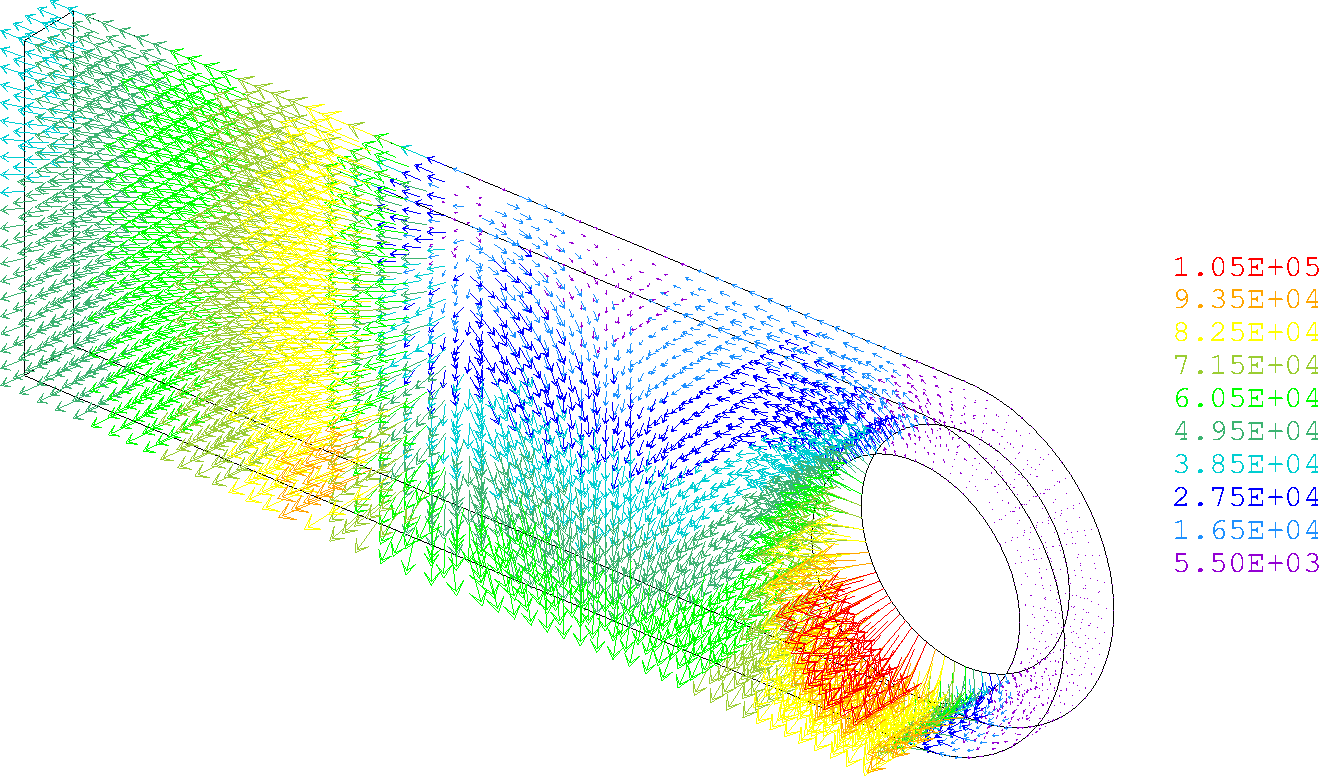
\includegraphics[width=4.7cm]{images/exo/4_flux}
    \end{textblock*}
    \item<2->\fe{Tracé de lignes d'iso valeurs}{Plotting iso vlaues lines}
    \onslide<2->{
      \lstinputlisting[language=gibiane, firstline=324, lastline=325]{dgibi/formation_debutant_2_thermique.dgibi}
      \begin{textblock*}{6cm}(6.7cm,0.1cm)
        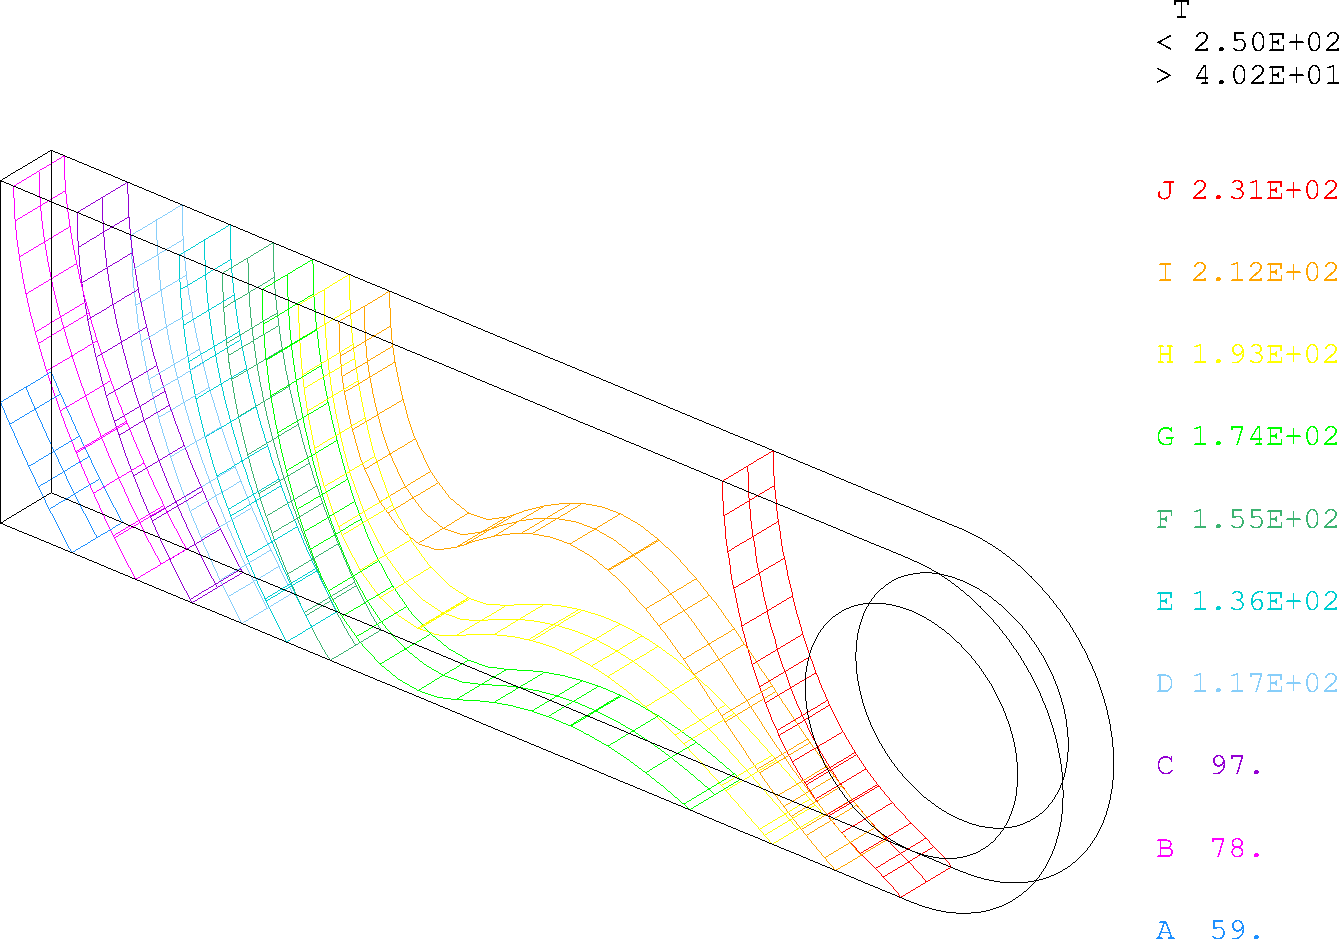
\includegraphics[width=4.7cm]{images/exo/4_temperatures}
      \end{textblock*}}
    \item<3->\fe{Retour au mode de tracé par défaut}{Back to default plot mode}
    \onslide<3->{
      \lstinputlisting[language=gibiane, firstline=326, lastline=326]{dgibi/formation_debutant_2_thermique.dgibi}}
  \end{itemize}
  \vspace{2cm}
\end{frame}

\begin{frame}{\fe{5 Problème étudié}{5 Problem description}}
  \begin{itemize}
    \item \gray{\fe{Conduction, régime transitoire}{Conduction, transient}}
    \begin{columns}
      \begin{column}{.4\textwidth}
        \item \gray{\fe{Température imposée}{Imposed temperature}}
      \end{column}
      \begin{column}{.4\textwidth}
        \item \gray{\fe{Flux de chaleur imposé}{Imposed heat flow}}
      \end{column}
    \end{columns}
    \begin{columns}
      \begin{column}{.4\textwidth}
        \item \gray{\fe{Convection}{Convection}}
      \end{column}
      \begin{column}{.4\textwidth}
        \item \gray{\fe{Source volumique}{Volume source}}
      \end{column}
    \end{columns}
    ~\\
    \item \fe{\ul{Rayonnement}}{\ul{Radiation}}\\
    \begin{center}
    \footnotesize
    \begin{tikzpicture}
      \node[anchor=south west,inner sep=0] (image) at (0,0)
      {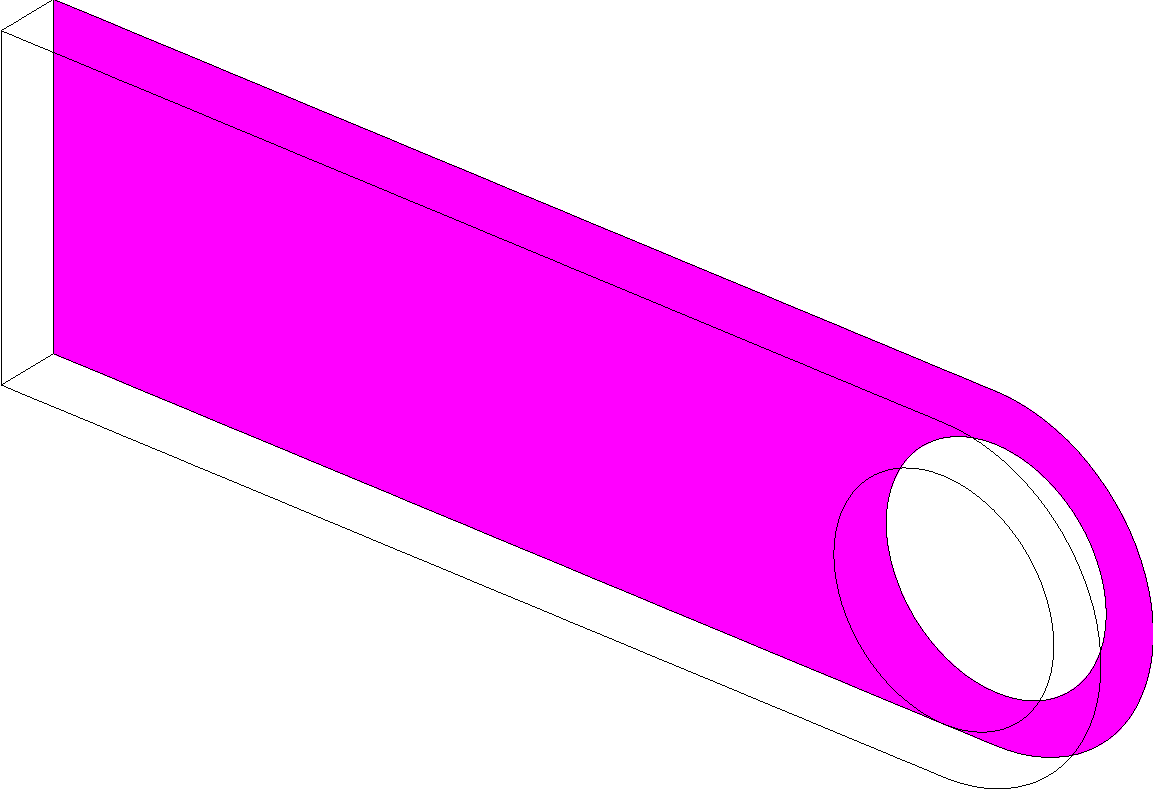
\includegraphics[width=3.5cm]{images/exo/5_cl_rayonnement}};
      \begin{scope}[x={(image.south east)},y={(image.north west)},color=magenta]
        \draw (0.7,0.9) node[anchor=north west] {$T_\infty$~=~-140~°C};
        \draw (0.7,0.75) node[anchor=north west] {$\varepsilon$~=~0.9};
      \end{scope}
    \end{tikzpicture}
    \normalsize
  \end{center}
  \end{itemize}
  \vspace{2cm}
\end{frame}

\begin{frame}{\fe{5 Thermique non linéaire}{5 Non linear thermal analysis}}
             {\fe{Transitoire, conduction, convection, source, rayonnement}
                 {Transient, conduction, convection, source, radiation}}
\begin{itemize}
    \item \fe{Objectif : calcul thermique transitoire non linéaire}
             {Objective: non linear transient thermal calculation}
    \begin{center}
      $[C]\{\dot{T}\}+[K]\{T\}=\{P(T)\}$
    \end{center}
    \item \fe{Méthode :}{Method:}\\
    \begin{tabular}{ll}
      \fe{ajout d'un modèle de rayonnement}{adding a radiation model}\\
      \fe{ajout d'un chargement de rayonnement}{adding a radiation load}
    \end{tabular}
  \end{itemize}
\end{frame}

\begin{frame}{\fe{5 Thermique non linéaire}{5 Non linear thermal analysis}}
             {\fe{Transitoire, conduction, convection, source, rayonnement}
                 {Transient, conduction, convection, source, radiation}}
  \begin{itemize}
    \item \fe{Nouveaux paramètres}{New parameters}
    \lstinputlisting[language=gibiane, firstline=57, lastline=58]{dgibi/formation_debutant_2_thermique.dgibi}
    \item \fe{Formulation mathématique (rayonnement)}{Mathematical formulation (radiation)}
    \lstinputlisting[language=gibiane, firstline=352, lastline=354]{dgibi/formation_debutant_2_thermique.dgibi}
    \item<2->\fe{Chargement température de rayonnement + description temporelle}
                {Load for radiation temperature + time description}
    \onslide<2->{
      \lstinputlisting[language=gibiane, firstline=356, lastline=358]{dgibi/formation_debutant_2_thermique.dgibi}}
  \end{itemize}
\end{frame}

\begin{frame}{\fe{5 Thermique non linéaire}{5 Non linear thermal analysis}}
             {\fe{Transitoire, conduction, convection, source, rayonnement}
                 {Transient, conduction, convection, source, radiation}}
  \begin{itemize}
    \item \fe{Résolution avec \kwo{PASAPAS}}{Solving with \kwo{PASAPAS}}\\
    \avous{\fe{Remplir la table pour \kw{PASAPAS} et résoudre}{Fill in the table for \kw{PASAPAS} and solve}}
    \onslide<2->{
      \lstinputlisting[language=gibiane, firstline=360, lastline=370]{dgibi/formation_debutant_2_thermique.dgibi}}
  \end{itemize}
\end{frame}

\begin{frame}{\fe{5 Thermique non linéaire}{5 Non linear thermal analysis}}
             {\fe{Transitoire, conduction, convection, source, rayonnement}
                 {Transient, conduction, convection, source, radiation}}
  \begin{itemize}
    \item \fe{Post traitement : coubres d'évolution temporelles}{Post processing: time curve}
    \lstinputlisting[basicstyle=\ttfamily\tiny, language=gibiane, firstline=375, lastline=378]{dgibi/formation_debutant_2_thermique.dgibi}
    \item<2->\fe{Tracé avec légende}{Plotting with a legend}
    \onslide<2->{
      \lstinputlisting[basicstyle=\ttfamily\tiny, language=gibiane, firstline=379, lastline=392]{dgibi/formation_debutant_2_thermique.dgibi}}
    \onslide<3->{
      \lstinputlisting[basicstyle=\ttfamily\tiny, language=gibiane, firstline=397, lastline=398]{dgibi/formation_debutant_2_thermique.dgibi}
      \begin{textblock*}{6cm}(6.3cm,-4.7cm)
        \begin{tikzpicture}
          \node[anchor=south west,inner sep=0] (image) at (0,0)
          {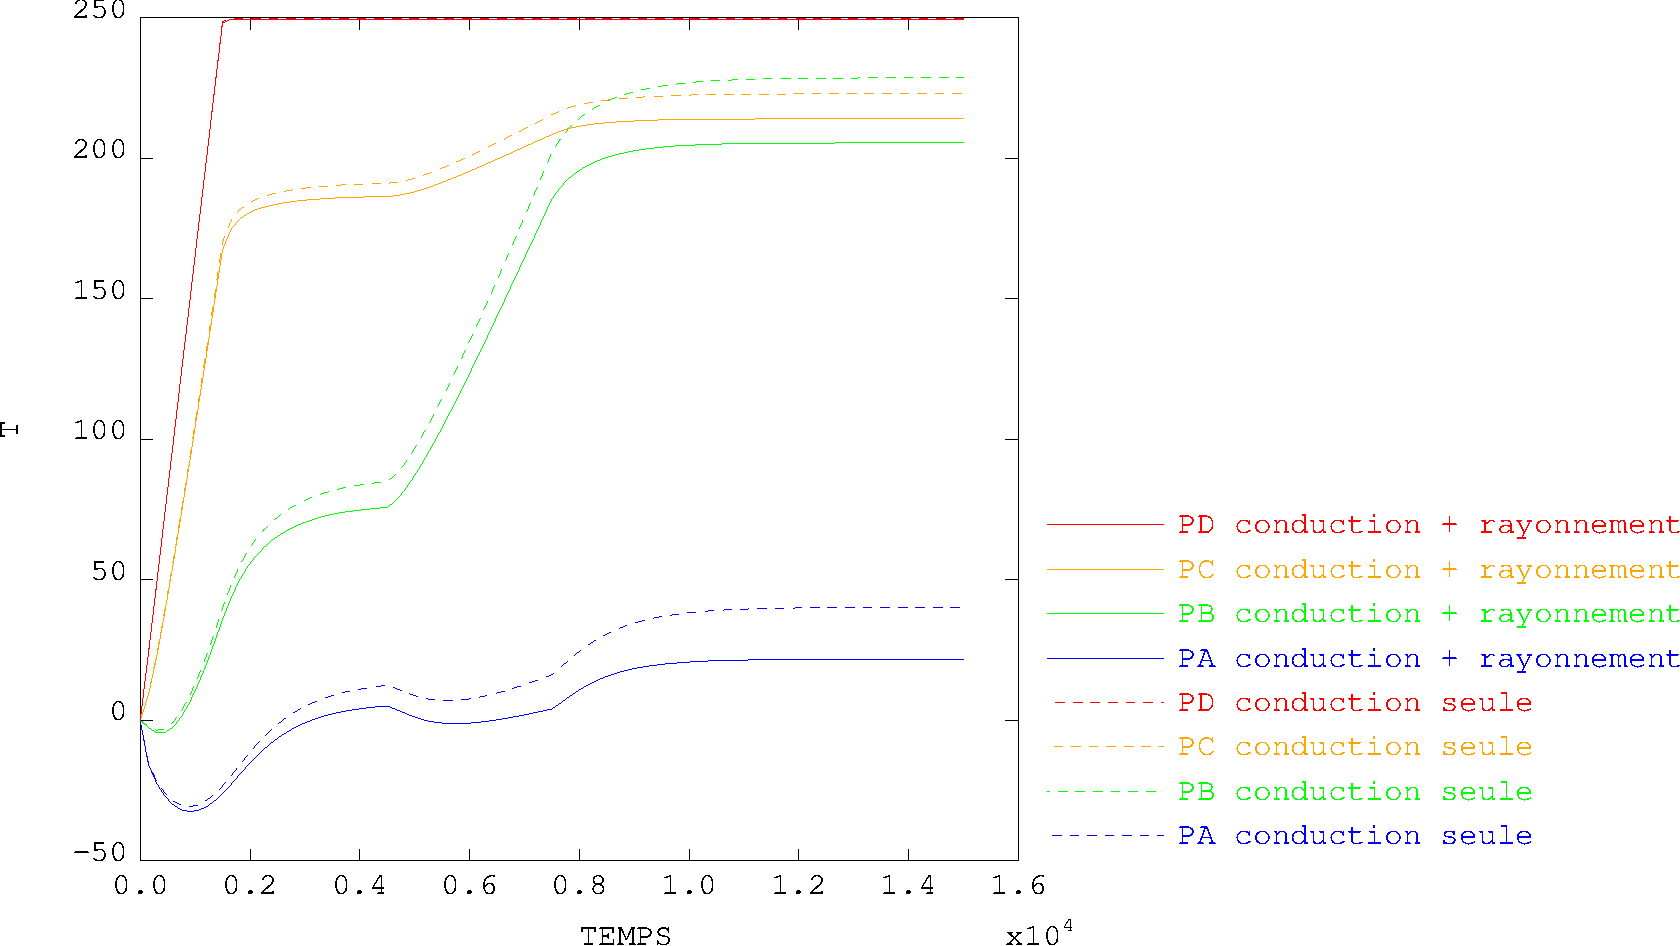
\includegraphics[width=6cm]{images/exo/5_evol_temperatures}};
        \end{tikzpicture}
      \end{textblock*}}
    \end{itemize}
\end{frame}

\begin{frame}{\fe{5 Thermique non linéaire}{5 Non linear thermal analysis}}
             {\fe{Transitoire, conduction, convection, source, rayonnement}
                 {Transient, conduction, convection, source, radiation}}
  \begin{itemize}
    \item \fe{Post traitement : boucle de tracés}{Post processing: loop for plot}
    \lstinputlisting[basicstyle=\ttfamily\tiny, language=gibiane, firstline=406, lastline=411]{dgibi/formation_debutant_2_thermique.dgibi}
    \lstinputlisting[basicstyle=\ttfamily\tiny, language=gibiane, firstline=413, lastline=413]{dgibi/formation_debutant_2_thermique.dgibi}
    \lstinputlisting[basicstyle=\ttfamily\tiny, language=gibiane, firstline=415, lastline=415]{dgibi/formation_debutant_2_thermique.dgibi}
    \begin{textblock*}{5cm}(6.2cm,-1.3cm)
      \animategraphics[controls,loop,poster=last,width=6cm]{10}{images/exo/5_temperatures.}{001}{101}
    \end{textblock*}
    \vspace{1cm}
    \item<2->\fe{Sauvegarde des données}{Saving data}
    \lstinputlisting[basicstyle=\ttfamily\tiny, language=gibiane, firstline=441, lastline=444]{dgibi/formation_debutant_2_thermique.dgibi}
  \end{itemize}
\end{frame}
